\section{Numerical experiments}\label{sec:exp}

In this section, we present numerical experiments to demonstrate the performance of~\ref{algo:AL} under different conditions. 
Among the three presented experiment, the first two use an analytical solution of the underlying PDE, while the third one is based on actual FE simulations of a PDE.
The choice of analytical forward models allows to evaluate the actual error and compare convergence rates and reduces the time required by realizations of~\ref{algo:AL}. 
At the end of the section, we will use the setup and data from the experiments to evaluate the influence of the estimation of the discretization noise's covariance on the quality of the GPR surrogate and of the GPR-based solution of the IP.  \medskip 

The remainder of this section is organized as follows: in Section~\ref{sec:setup}, we describe the objectives of the experiments and general setup across them; Section~\ref{sec:implementation} provides implementation details; in Section~\ref{sec:3dexp}, we present an analytical example with 3d parameter space based on the Poisson equation; in Section~\ref{sec:6dexp}, we present an analytical example with 6d parameter space based on the diffusion equation; in Section~\ref{sec:FEexp}, we present a FE example based on elastomechanics with 2d parameter space; finally, in Section~\ref{sec:cov-est}, we elaborate data from the previous experiments to assess the impact of noise covariance estimation.

\subsection{Objectives and general setup}\label{sec:setup}

The experiments aim at testing the proposed strategy on low to moderate-dimensional parameter spaces.
The scope of these examples can be articulated in three senses:
\begin{enumerate}
    \item comparing the training strategy as compared to other strategies for the same surrogate model;
    \item comparing the performance of LR surrogates to the more established GPR surrogate models across different training strategies;
    \item comparing the effect on GPR of discretization noise estimation as given by Equation~\eqref{eq:shrinkage-estimator} in Section~\ref{sec:GPAL}.
\end{enumerate}
While the first and the last points can be evaluated more easily, the second point is more difficult to evaluate as it requires a fair comparison between the two kinds of surrogate models.
Consequently for point 2, we will exploit the available ground-truth in the analytical examples, while for the FE example we will resort to a qualitative comparison.

Unlike the experiments in~\cite{VillaniArconesUngerWeiser2025}, where various setups for the budget fractionating and the FE cost depending on the fraction $\frac{l}{r}$ were considered, in this work we fix them and do not investigate their effect on the performance of the algorithm.
Previous works~\cite{SemlerWeiser2023,VillaniArconesUngerWeiser2025,VillaniUngerWeiser2024} have shown that the effect of an higher FE cost is to reduce the effectiveness of tolerance optimization, resulting in performances similar to those of a fixed tolerance strategy.

As a benchmark, we consider the non-adaptive space-filling approach given by Latin Hypercube Sampling (LHS)~\cite{McKayBeckmanConover1979} and an approach similar to the one proposed in~\cite{Dinkel2024}, which also relies on interleaved sampling but selects the candidates randomly from the current posterior approximation, both using fixed tolerances.
Moreover, we also consider the fixed tolerance version of the proposed strategy, which is given by~\ref{algo:AL} without the tolerance optimization step. 
For the GPR surrogate, we name the strategy of~\ref{algo:AL} \texttt{AGP} for adaptive Gaussian process, the fixed tolerance version \texttt{posAdGP} for position-adaptive Gaussian process, the strategy randomly drawing new points from the posterior \texttt{randGP} and the LHS strategy \texttt{LHSGP}.
Similarly, we will refer to the LR surrogate training strategy of~\ref{algo:AL} as \texttt{ALR}, to the fixed tolerance version as \texttt{posAdLR}, to the LR-based version of the strategy randomly drawing from the posterior as \texttt{randLR} and to the LR-based LHS approach as \texttt{LHSLR}. \medskip

In all experiments, the measured quantity is directly obtained from point-wise evaluations $u(\theta;p)$ of the equation's solution $u$, for $\theta$ in a set of sensors $\mc S$; consequently, the measurement operator $H$ is given by
\[
    H(u(\cdot; p)) = \left( u(\theta_j;p)\right)_{j=1,\ldots, \text{dim} \mc Y} \ \text{ for some ordering } \ \theta_1, \ldots, \theta_{|\mc S|} \ \text{ of the sensors } \ \mc S.
\]
In the analytical examples $u(\theta;p) \in \R$, while for the FE example $u(\theta;p)\in \R^3$: in the latter case, only one component of the displacement is assumed to be measured in each sensor. \medskip

For the analytical examples the analytical formula of a solution is available and no discretization is necessary.
This allows us to evaluate the forward model $y(p)$ with close to zero cost, rendering it possible to represent the ground-truth posterior and to perform repeated runs of the algorithm. 
On the downside, this requires us to simulate the discretization error; we do so by adding by adding pseudorandom noise $\nu$ with the appropriate distribution to forward model evaluations $y(p)$. \newline
When training GPR surrogates, we consider zero mean Gaussian noise $\nu \sim \mc N (0, \tau^2 \Sigma_T^2)$ when simulating $y_\tau(p)$, where \[
\big(\Sigma_T\big)_{ij} = \sigma\big( \|\theta_i - \theta_j\|_{\mc Y} \big) \ \text{ for } \ \theta_i, \theta_j \in \mc S
\]
with $\sigma$ the probability density function of the centered normal distribution $\mc N(0, \frac{1}{2})$.
Such a setup allows us to evaluate the effect of the discretization noise on the GPR surrogate model.\newline
When training LR surrogates, we consider uniform noise $\nu \sim \mc U([-\tau, \tau]^{\text{dim} \mc Y})$ so that $I_\tau$ is an interval and the assumptions of propositions~\ref{prp:LR-PI},~\ref{prp:LR-likelihood} and~\ref{prp:EER} are met. \newline
In order to compensate for the lack of discretization noise and to evaluate the sensitivity of the algorithms to randomness, we will perform and average repeated runs of the algorithm with the same budget but different random seeds.
Details about the number of runs will be given in the respective sections. \medskip

For GPR, we consider a separable RBF kernel 
\[
    k_{(\mathbf{L}, \lambda)}(p, p') =  \exp ( - \norm{p - p'}^2_{\mathbf{L}} ) \ K_\lambda,
\]
as introduced by equations~\eqref{eq:separable-kernel} and~\eqref{eq:RBF-kernel}, with diagonal $\mathbf{L} = \text{diag}(\ell_1, \dots, \ell_{\text{dim} \Theta})$, $\lambda = (\mathbf{s}, \mathbf{C}) $ and
\[
K_\lambda = \text{diag}(\mathbf{s}) + \mathbf{CC}^T,
\] 
where $\mathbf{s} \in \R^{\text{dim} \mc Y}$ is a scaling vector and $\mathbf{C} \in \R^{\text{dim} \mc Y \times 2}$ is a rank 2 matrix which models the correlation among components. 
Moreover, to stabilize the hyperparameters we consider a Gamma prior $\mc G(2, 10)$ for the lengthscales $\ell_1, \dots, \ell_{\text{dim} \Theta}$ and impose a constraint $\ell_i > 10^{-1}$ for all $i$.

For LR, we consider the euclidean norm $\norm{\cdot}_2$ on the parameter space $\Theta$ and set the Lipschitz constant estimation hyperparameter $\lambda$ in Equation~\eqref{eq:lips-const} to 
\[ \lambda = 1.1 + \exp{\left(-\frac{n_\text{train}}{\text{dim} \Theta^2}\right)},\] where $n_\text{train}$ is the number of training points.
\medskip

To produce a MCMC representation of the posterior, we consider Ensemble Sampling as introduced in Section~\ref{sec:IP-sol} using at each step a move selected randomly among the stretch move~\eqref{eq:stretch-move}, the walk move~\eqref{eq:walk-move} and the DIME move from~\cite{Boehl}, with probabilities 0.25, 0.25, 0.5 respectively. 
When initializing the sampler, we randomly select an initial state through LHS and then we perform burn-in sampling, testing the convergence of the sampler through the Gelman-Rubin statistic $\hat R$ defined in Equation~\eqref{eq:hatR} every 100 iterations.
\medskip

In this work, we fix some parameters of~\ref{algo:AL} across different experiments, while others are set according to the specific problem.
Regarding sampling, the number $n_w$ of walkers in the ensemble is selected depending on the dimensionality of the problem; the posterior is not sampled at every iteration but every $N_{\text{sample}}$ iterations: at iteration $j$, the number of samples to be drawn $d_j$ and the number of samples to be burned $b_j$ at Step 1 are given by
\[
d_j = b_j = \begin{cases}
    250 \cdot n_w \cdot  & \text{ if } j \equiv 1 \mod N_{\text{sample}} \\
    0 & \text{ otherwise}
\end{cases}.
\]
By this, whenever we sample the posterior we rebuild a totally new chain $\mc S_j$. 
Moreover, after the required accuracy level is reached, we stop the algorithm and sample the posterior with a larger number of samples $d_{J_{\max} +1} = 500 \cdot n_w$, while burning the previous $b_{J_{\max} +1} = 250 \cdot n_w$ samples.\newline
We consider a single candidate point at each iteration, selecting the global maximum of the acquisition function~\eqref{eq:acq-fun-disc}, $s_j = 1$ at Step 2 of~\ref{algo:AL}; regarding the budget $\Delta W_j$ for the tolerance optimization problem at Step 3, we consider a default tolerance $\tau$ and assign the budget $\Delta W_j = \tau^{-\frac{l}{r}}$ to the optimization problem, where $l$ and $r$ are the FE cost parameters.
We consider non uniform budget fractionating, adapting the computational budget for Problem~\eqref{prob:incremental-doe} to the convergence status by halving the default tolerance if the target quantity does not reduce adequately in $N_\text{sample}$ iterations; we set the fraction $\frac{l}{r}$ to $1$ for the analytical examples and to $1.5$, corresponding to quadratic FE $r=2$ on a 3d mesh $l=3$, for the elastomechanics example.  \newline
Finally, the tolerance level \texttt{tol} is selected to be proportional to the measurement's covariance for the GPR surrogate and to the measurement's standard deviation for the LR surrogate, as the error estimates are related to the surrogate's covariance and standard deviation respectively.\medskip

\subsection{Implementation details}\label{sec:implementation}
A Python implementation of~\ref{algo:AL}, available at \footnote{\url{git.zib.de/pvillani/thesis}} along with the results, has been developed to conduct the experiments on an Intel Core i7-9700T × 8 CPU. \medskip

The Gaussian process surrogate model uses a GPyTorch~\cite{GPyTorchPaper} base model, set to work with double-precision floating-point numbers.
GPyTorch's Adam is employed to optimize the hyperparameters on the marginal likelihood~\eqref{eq:marginal-likelihood}. \medskip

The two optimization problems to determine new candidate points and evaluation tolerances are solved through the SciPy optimizer \texttt{scipy.optimize.minimize}. 
For the GPR acquisition function, the exact gradient is not available and local maxima of~\eqref{eq:acq-fun-disc} are found using the L-BFGS-B algorithm~\cite{ZhuBirdNocedal}. 
As derivative information is available for the LR acquisition function~\eqref{eq:alpha-LR} and for the target of the tolerance problem, we employ the Sequential Least Squares Quadratic Programming (SLSQP) algorithm to solve Problem~\eqref{prob:discrete-tol} and to find maximizers of~\eqref{eq:acq-fun-disc} for a LR model. 
For tolerance optimization, before applying the SLSQP algorithm a coordinate transformation is applied in order to linearize the work constraint. 
In all cases, we adopt a multi-start approach by selecting a number of initial points through a low-discrepancy sequence. \medskip

To sample the posterior, we utilize the \texttt{emcee}~\cite{emceePaper} implementation of Ensemble Sampling. The posterior plots are then realized using the \texttt{corner} package~\cite{corner}. \medskip

While the interface for the experiments is also realized in Python, the FE model is implemented in C++17 through the \texttt{Kaskade 7} Finite Element toolbox~\cite{GoetschelSchielaWeiser2021}.\medskip

The rest of the implementation has been developed by the author and relies in particular on the \texttt{numpy} package~\cite{numpy}, while the \texttt{matplotlib} package~\cite{matplotlib} has been employed for the generation of plots. 

\subsection{3d analytical example - Poisson equation}\label{sec:3dexp}

The first numerical experiment involves the distributional Poisson equation on $\R^3$
\[
 \Delta u = \delta_{x_0}
\] 
with a Dirac's delta source centered in some $x_0 \in \R^3$.
As discussed in Section~\ref{sec:PDE}, the fundamental solution of the Laplace equation~\eqref{eq:Poisson-fundamental-solution} can be interpreted as the solution of such equation; this leads us to consider as a solution
\[
u(x; x_0) =  \frac{1}{2 \|x-x_0\|_2},
\]
where a multiplicative constant has been added for numerical stability reasons. \medskip

To formulate an IP, $x_0$ is assumed to be an unknown parameter and we aim at identifying it by measurements of $u(x;x_0)$ in sensors $x \in \mc S$ for 
\[
    \mc S = \left\{
        \begin{pmatrix}
            \cos( i \frac{\pi}{3}) \sin( j \frac{\pi}{2}) \\
            \sin( i \frac{\pi}{3}) \sin( j \frac{\pi}{2}) \\ 
            \cos( j \frac{\pi}{2})
        \end{pmatrix} 
        \in \R^3 \ \Big| \ i \in \{0,1,2,3,4,5\}, \ j \in \{0,1,2,3\}
     \right\},
\]
resulting in 14 sensors on the unit sphere and consequently a 14-dimensional measurement space $\mc Y = \R^{14}$. \newline
The parameter space is assumed to be $\Omega = \left[-\frac{1}{2}, \frac{1}{2}\right]^3$ and a Normal prior $\mc N (0, \frac{1}{4}I_3)$ is considered.

We generate measurements by adding pseudorandom noise $N \sim \mc N (0, \sigma^2 I_{14})$, with $\sigma = 10^{-2}$ to the exact forward model evaluations $y(p)$ for some $p$. 
We consider 5 different measurements corresponding to 5 different $p$ randomly extracted from the prior distribution and, as the discretization error is simulated, we perform 5 runs of each training strategy with different random seeds for each measurement.
\medskip

For the GPR surrogate, we consider a default configuration with a halting threshold $\texttt{tol} = \sigma^2 \cdot \frac{\text{dim} \mc Y }{20} = 7\cdot 10^{-5}$, where the factor $\frac{\text{dim} \mc Y}{20}$ is chosen to be proportional to the number of output components of the surrogate model, as the error model sums the predictive variance over the output components, and divided by a factor 20 to impose the surrogate model's variance to be smaller than the measurement's variance.
For all measurements and seeds, we sample every $N_{\text{sample}} = 3$ iterations and we set the number of walkers to $n_w = 32$.
We begin with an initial design of $5$ points selected through LHS and with default tolerance $\tau_d = 3 \cdot 10^{-2}$, and we perform a maximum of $J_{\max} = 10 \cdot N_{\text{samples}} = 30$ iterations; when assigning the budget $\Delta W_j = \tau ^{-\frac{l}{r}}$ to the optimization problem, we use the default value $\tau= \tau_d$ for the first $2\cdot N_{\text{samples}} = 6$ iterations and then every $N_{\text{sample}}$ iterations we halve it if the expected error has not reduced by a factor 4 compared to the $N_{\text{sample}}$-th latest iteration, i.e. if $\frac{E(D(\mc D_j))}{E(D(\mc D_{j-N_{\text{sample}}}))} > \frac{1}{4}$.

\begin{figure}[H]
\begin{center}
    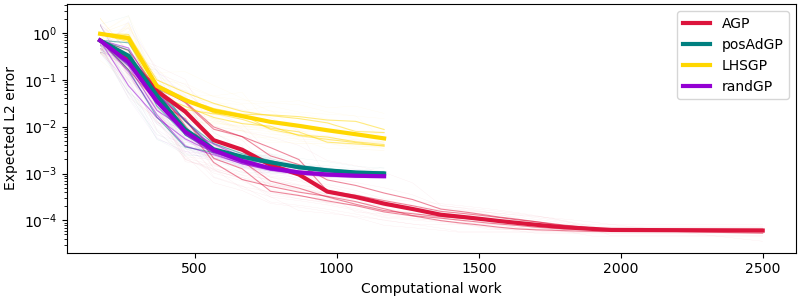
\includegraphics[width=0.8\textwidth]{results/pictures/d3/GP_res.png}
\end{center}
\caption{Convergence rates for the GPR expected error over computational budget for the four considered strategies on the 3d example and default configuration. The thinner lines represent a single run, the lines of median thickness represent the average over the 5 random seed for each measurement and the thickest lines represent the average over the whole 25 runs.}
\label{fig:3dGPconv}
\end{figure}

This setup results in the expected error per spent budget curves represented by Figure~\ref{fig:3dGPconv} for the different training strategies.
We see that, while \texttt{LHSGP} struggles to reduce the expected error and has a slower convergence rate, the fixed-tolerance strategies \texttt{posAdGP} and \texttt{randGP} are able to perform on par with \texttt{AGP} until they hit a plateau around an error level of $10^{-3}$, while \texttt{AGP} is able to reach the threshold $\texttt{tol}$ before the maximum number of iterations.
Moreover we observe that in this case random selection of the candidates in \texttt{randGP} is as effective as the position-adaptive strategy \texttt{posAdGP}, resulting in a similar convergence velocity.

\begin{table}[H]
    \begin{centering}
    \begin{tabular}{cccc}
    \toprule
         & Iterations & Training points & Computational work \\
         \midrule
         \texttt{AGP} 
         & 15.1 & 14.4 & 830 \\
         \texttt{posAdGP} 
         & 19.2 & 24.2 & 806 \\
         \texttt{randGP} 
         & 18.8 & 23.8 & 794  \\
         \bottomrule
    \end{tabular}
    \caption{Average over the 25 runs of number of iterations, points in the training set and computational work required to reduce the expected error below $2 \cdot 10^{-3}$ for the GPR-based adaptive strategies.}
    \label{tab:3dGP-plateau}
\end{centering}
\end{table}

As shown in Table~\ref{tab:3dGP-plateau}, while before the plateau \texttt{AGP} and the position-adaptive strategies achieve a similar performance in terms of expected error per budget, \texttt{AGP} uses a smaller number of iterations and training points as it adaptively reduces the default tolerance $\tau_d$ and optimizes work distribution.

\begin{table}[H]
    \begin{centering}
        
    
    \begin{tabular}{ccccccccccc}
    \toprule
        & Converged & $W$  & \multicolumn{4}{c}{Training points} & \multicolumn{4}{c}{Iterations} \\ 
        &   &  avg  & avg   & med   & min   & max   & avg   & med   & min   & max \\
        \midrule
        \texttt{AGP}, $\tau_d = 3 \cdot 10 ^{-2}$    
        &always & 1830 & 15.3  &  15   &  12   &  20   &  20.6 &  21   &   16  & 23   \\
        Others, $\tau_d = 3 \cdot 10 ^{-2}$    
        & never & 1167 &  35   &  35   &  35   &   35  &   30  &  30   &   30  & 30   \\
        \texttt{posAdGP}, $\tau_d = 10 ^{-3}$ 
        & always&14320 & 14.3  &  15   &  12   &   18  &  9.3  &  10   &   7   & 13   \\
        \texttt{randGP}, $\tau_d = 10 ^{-3}$ 
        & always&15080 & 15.1  &  14   &  14   &   17  &  8.1  &  9    &   9   & 12 \\
        \texttt{LHSGP}, $\tau_d = 10 ^{-3}$ 
        & never &35000 &  35   &  35   &  35   &   35  &   30  &   30  &   30  & 30   \\
    \bottomrule
    \end{tabular}
    \caption{Status of the training after the final iteration of different strategies and configurations for the GPR surrogate, 3d example. For the total computational work $W$ the average over the 25 runs is provided, while for the final number of points in the training set and the number of iterations necessary to terminate the training the average, the median, the minimum and the maximum are provided.
    }
    \label{tab:3dGP-recap}
\end{centering}
\end{table}

The plateau phase motivates us to test the behavior of the fixed-tolerance strategies with a lower tolerance $\tau_d = 10^{-3}$: in this case \texttt{posAdGP} and \texttt{randGP} are able to reach the target threshold $\texttt{tol}$ as shown in Figure~\ref{fig:3dGP-other}, but they require a larger computational budget and a similar number of training points as \texttt{AGP} with the lower default tolerance $\tau_d =  3\cdot 10^{-2}$, see Table~\ref{tab:3dGP-recap}.
We observe that even in this higher-accuracy case, \texttt{LHSGP} is unable to reach the convergence threshold \texttt{tol}.
Finally, on Table~\ref{tab:3dGP-recap} we can notice that on average a run \texttt{AGP} does not include the selected candidate in 10 iterations, resulting in an average number of 15.3 points in the design, of which 5 are the initial ones, over 20.6 average iterations.
As the computational costs of GPR scale with the number of training points, a reduced number of training points renders the evaluation of the surrogate more efficient.

\begin{figure}[H]
\begin{center}
    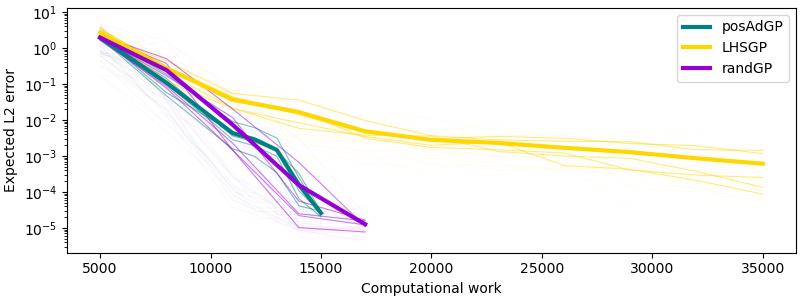
\includegraphics[width=0.8\textwidth]{results/pictures/d3/config_dtol0.001/GP_res.png}
\end{center}
\caption{Convergence rates for the GP expected error over computational budget for the fixed-tolerance strategies, default tolerance $\tau_d = 10^{-3}$. The thinner lines represent a single run, the lines of median thickness represent the average over the 5 random seed for each measurement and the thickest lines represent the average over the whole 25 runs.}
\label{fig:3dGP-other}
\end{figure}

For the LR surrogate, we consider a halting threshold $\texttt{tol} = \sigma \cdot \frac{\text{dim} \mc Y }{1.5} = 9.\bar 3 \cdot 10^{-2}$, proportional to the measurement's standard deviation as the error model is based on the standard deviation of the LR surrogate.
For LR, we sample every $N_{\text{sample}} = 4$ iterations and we set the number of walkers to $n_w = 32$.
The initial design consists of 5 points selected through LHS and with default tolerance $\tau_d = 3 \cdot 10^{-2}$, and we perform a maximum of $J_{\max} = 8 \cdot N_{\text{samples}} = 32$ iterations; when assigning the budget $\Delta W_j = \tau ^{-\frac{l}{r}}$ to the tolerance optimization problem at Step 3, we use the default value $\tau= \tau_d$ for the first $2\cdot N_{\text{samples}}= 8$ iterations and then every $N_{\text{sample}}$ iterations we halve it if the expected error has not reduced by a factor 2 compared to the $N_{\text{sample}}$-th latest iteration, i.e. if $\frac{E(D(\mc D_j))}{E(D(\mc D_{j-N_{\text{sample}}}))} > \frac{1}{2}$.
The different choices regarding configuration parameters as compared to GPR are due to the higher prediction variance and lower sensitivity of the LR surrogate model to computational work. 

\begin{figure}[H]
\begin{center}
    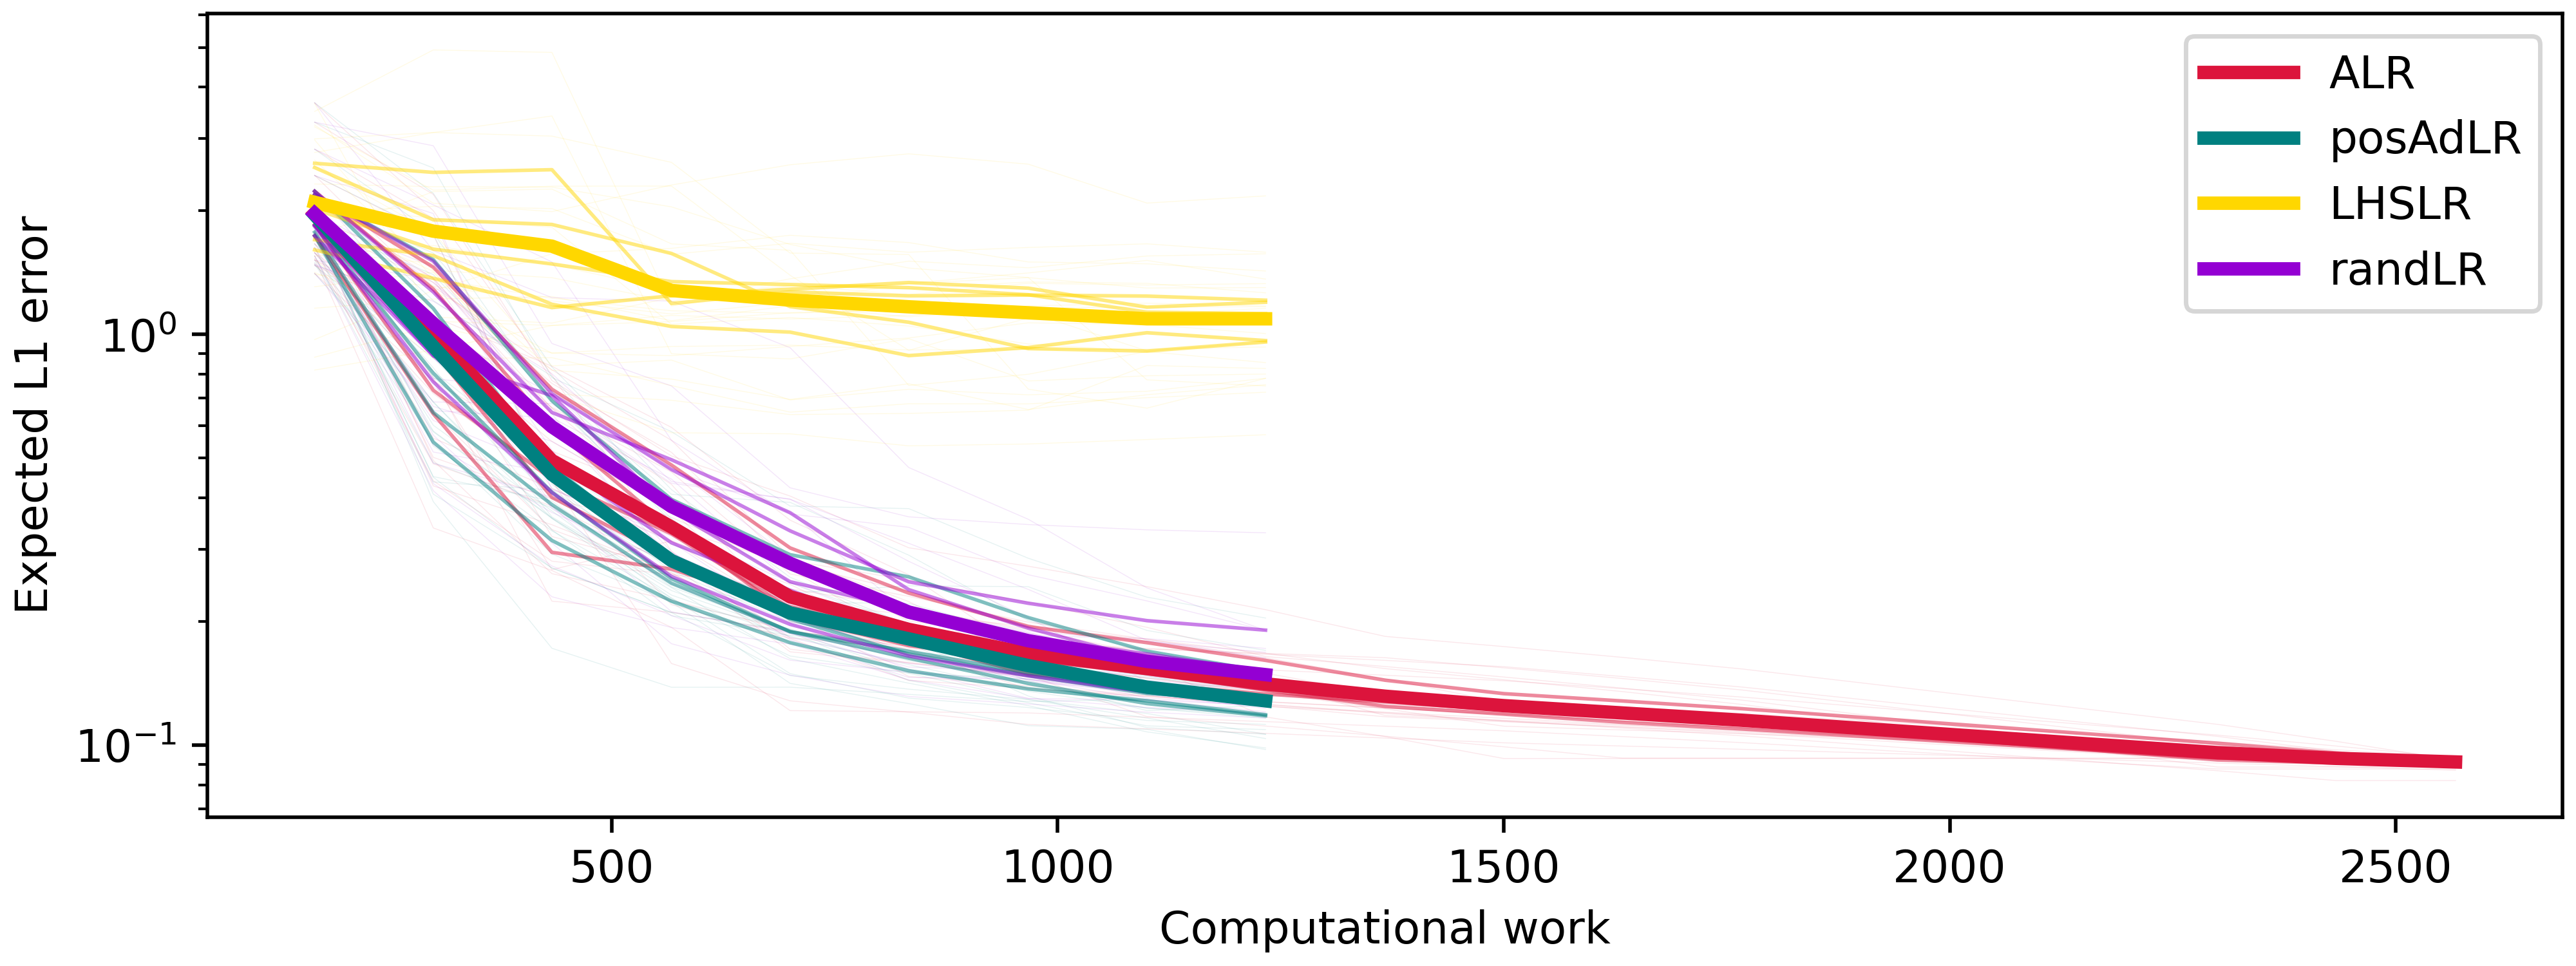
\includegraphics[width=0.8\textwidth]{results/pictures/d3/LR_res.png}
\end{center}
\caption{Convergence rates for the LR expected error over computational budget for the four considered strategies. The thinner lines represent a single run, the lines of median thickness represent the average over the 5 random seed for each measurement and the thickest lines represent the average over the whole 25 runs.}
\label{fig:3dLRconv}
\end{figure}

Figure~\ref{fig:3dLRconv} depicts the expected error per budget curves for the different training strategies. 
We observe that, as opposed to the GPR surrogate, the fixed-tolerance strategies \texttt{posAdLR} and \texttt{randLR} perform on par with \texttt{ALR} until they meet the maximum number of iterations, while \texttt{ALR} is able to reach the target threshold $\texttt{tol}$ before the maximum number of iterations thanks to the adaptive budget allocation.
It is worth noting that \texttt{LHSLR} performs significantly worse than the other strategies, barely reducing the expected error at all, while \texttt{posAdLR} performs slightly better than \texttt{randLR}. 
In this case, the fully adaptive strategy \texttt{ALR} includes the new candidate in the design more frequently than \texttt{AGP}, resulting in an average for the 25 runs of 27.1 training points over 26.4 iterations, corresponding on average to around 4 iterations without the inclusion of the candidate.
This fact, as well as the effectiveness of fixed-tolerance strategies, suggests that for LR the inclusion of high-accuracy points is a less relevant factor than in GPR on this example. \medskip

\begin{table}[H]

    \begin{centering}
        
    \hspace*{-1.5cm}
    \begin{tabular}{ccccccccccccc}
    \toprule
        & \multicolumn{4}{c}{MAP error}  & \multicolumn{4}{c}{Posterior mean error} & \multicolumn{4}{c}{Posterior st. dev. error} \\ 
        & \multicolumn{4}{c}{$ \|p_\text{MAP} - \hat p _\text{MAP}\|_2 $}  & \multicolumn{4}{c}{$ \|p_\text{mean} - \hat p _\text{mean}\|_2 $} & \multicolumn{4}{c}{$\| \text{diag}(\Sigma_P) - \text{diag}( \hat \Sigma _P) \|_2$} \\ 
        & avg   & med   & min   & max   & avg   & med   & min   & max   & avg   & med   & min   & max \\
        \midrule
        \texttt{AGP}
        & 0.0046 & 0.0039 & 0.0011 & 0.0086
        & 0.0037 & 0.0036 & 0.0011 & 0.0084
        & 0.0038 & 0.0015 & 0.0001 & 0.0131 \\
        \texttt{posAdGP}
        & 0.0145 & 0.0152 & 0.0048 & 0.0214 
        & 0.0136 & 0.0141 & 0.0049 & 0.0217
        & 0.0071 & 0.0067 & 0.0034 & 0.0110 \\
        \texttt{randGP}
        & 0.0103 & 0.0097 & 0.0048 & 0.0192 
        & 0.0107 & 0.0106 & 0.0041 & 0.0201
        & 0.0064 & 0.0058 & 0.0011 & 0.0136 \\
        \texttt{LHSGP}
        & 0.0332 & 0.0325 & 0.0124 & 0.0753 
        & 0.0312 & 0.0278 & 0.0119 & 0.0658
        & 0.0149 & 0.0131 & 0.0088 & 0.0331 \\
        \texttt{ALR}
        & 0.0186 & 0.0180 & 0.0041 & 0.0446
        & 0.0113 & 0.0102 & 0.0043 & 0.0272
        & 0.0094 & 0.0087 & 0.0024 & 0.0196 \\
        \texttt{posAdLR}
        & 0.0199 & 0.0178 & 0.0041 & 0.0524
        & 0.0139 & 0.0115 & 0.0037 & 0.0369
        & 0.0103 & 0.0095 & 0.0049 & 0.0208 \\
        \texttt{randLR}
        & 0.0225 & 0.0211 & 0.0077 & 0.0507
        & 0.0156 & 0.0141 & 0.0053 & 0.0283
        & 0.0117 & 0.0113 & 0.0052 & 0.0232 \\
        \texttt{LHSLR}
        & 0.1315 & 0.1134 & 0.0536 & 0.2801 
        & 0.1053 & 0.0992 & 0.0319 & 0.1988
        & 0.0717 & 0.0707 & 0.0251 & 0.1378 \\
        
    \bottomrule
    \end{tabular}

    \caption{Average, median, minimum and maximum of the absolute error on the MAP estimate, posterior mean and posterior standard deviation on each component over the 25 runs with default configuration.
    The analytical ground truth posterior and corresponding samples are utilized to compute the true MAP $p_\text{MAP}$, mean $p_\text{mean}$ and component-wise standard deviation $\text{diag}(\Sigma_P)$, while for each strategy the surrogate-based posteriors and samples are used to compute $\hat p_\text{MAP}$, $\hat p_\text{mean}$ and $\text{diag}(\hat \Sigma_P)$.
    }
    \label{tab:3d-comparison}
    \end{centering}
    
    
\end{table}

We compare the performance of the GPR and LR surrogates utilizing the available ground truth.
Table~\ref{tab:3d-comparison} shows the average error on the MAP estimate, posterior mean and posterior standard deviation of the different strategies and different surrogates.
First, we observe that the GPR-based strategies perform significantly better than the LR-based ones, with \texttt{AGP} being the best performing strategy across all metrics with a precision of one order of magnitude better than others on the MAP and mean errors. 
The tolerance-adaptive strategy \texttt{ALR} performs at a level similar to that of \texttt{posAdGP} and \texttt{randGP}, but with a higher computational cost.
As already noticed with the expected error per budget curves, the difference among \texttt{ALR} and the LR-based fixed-tolerance strategies is less pronounced than for GPR.
In fact, in the fixed-tolerance strategies LR is able to reach a performance at the same order of magnitude as GPR by having a locally-accurate representation of the forward model with a similar computational cost.
We can notice that the LHS-based strategies \texttt{LHSGP} and \texttt{LHSLR} are worst performing ones and display a remarkable performance difference between the two surrogate kinds. 
In this example, LR is unable to obtain a good approximation of the posterior through a globally-accurate surrogate, while GPR is able to reach a good approximation of the posterior even with a non-adaptive globally-accurate surrogate.
\begin{figure}[t]
\begin{center}
    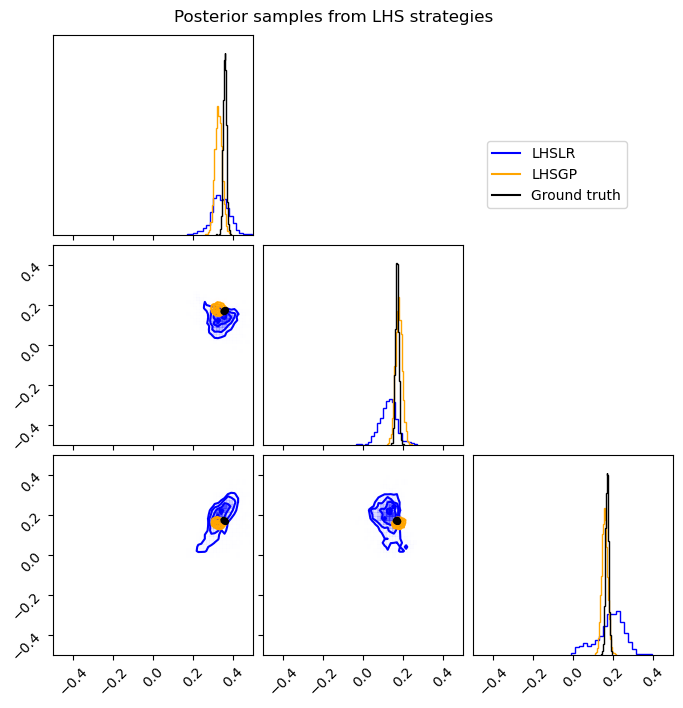
\includegraphics[width=0.8\textwidth]{results/pictures/d3/LHS_samples4_0.png}
\end{center}
\caption{Final sample chains from \texttt{LHSGP} and \texttt{LHSLR}, default tol $\tau_d = 3\cdot 10^{-2}$, compared with the ground truth for the run with the 5-th measurement set and pseudorandom seed 0.}
    \label{fig:3d-LHS}
\end{figure}
Figure~\ref{fig:3d-LHS} plots the samples gathered from the posteriors from \texttt{LHSGP} and \texttt{LHSLR} as well as the ground truth for one of the runs.




\subsection{6d analytical example - Diffusion equation}\label{sec:6dexp}

The second numerical experiment involves the homogeneous diffusion equation on $\R^3$ with unit diffusivity constant and no source
\[
\partial_t u - \Delta u =0,
\]
and initial conditions given by two Dirac's delta of opposite sign centered in some $x_p$ and $x_n$:
\[
f (0,x; x_p, x_n) = \delta(x-x_p) - \delta(x-x_n).
\]
We consider the difference of fundamental solutions of the diffusion equation centered in $x_p$ and $x_n$, scaled for numerical stability of the surrogates, as a solution of the above problem
\begin{equation}\label{eq:diffusion-solution}
f(t,x; x_p, x_n) = \frac{50}{(4 \pi t)^{\frac{3}{2}}} \left( \exp \left( - \frac{\norm{x-x_p}_2^2}{4t}\right)- \exp \left( - \frac{\norm{x-x_n}_2^2}{4t}\right) \right).
\end{equation}
We treat $x_p, x_n$ as unknown parameters and want to identify them by measuring $u(t,x;x_p, x_n)$ for $t,x \in \mc S$, where $\mc S$ is a set of times in $\R^+$ coupled with sensors in $\R^3$ given by
\[
\mc S  = \left\{ (t,x) \in \R^+ \times \R^3 \ \Big| \ t = 0.3, 0.5 \ \text{ and } \ x = \begin{pmatrix}
            \cos( i \frac{2\pi}{3}) \sin( j \frac{\pi}{4}) \\
            \sin( i \frac{2\pi}{3}) \sin( j \frac{\pi}{4}) \\ 
            \cos( j \frac{\pi}{4})
        \end{pmatrix} 
         \text{ for } i \in \{0,1,2\}, \ j \in \{0,1,2,3,4\}
        \right\}.         
\]
This results in 15 sensors at 2 different times, resulting in a 30-dimensional measurement space $\mc Y = \R^{30}$. \newline
As a parameter space, $\Omega = [-1,1]^6$ is considered and a Normal prior $\mc N (0, \frac{1}{4}I_6)$ is assumed.
Measurements are generated by exact forward model evaluations $y(p)$ for 4 different values of $p$ randomly extracted from the prior distribution, to which pseudorandom noise $N \sim \mc N (0, \sigma^2 I_{30})$, with $\sigma = 2 \cdot 10^{-2}$ is added.
For each of the 4 measurements, we perform 3 runs of each training strategy with different random seeds. \medskip

The configuration parameters for the GPR surrogate are similar to those of the previous example: we choose an halting threshold of $\texttt{tol} = \sigma^2 \cdot \frac{\text{dim} \mc Y }{20} = 6\cdot 10^{-4}$; sampling is performed every $N_{\text{sample}} = 4$ iterations, with an ensemble comprising of $n_w = 64$ walkers.
The initial design consists of 13 points selected through LHS with default tolerance $\tau_d = 3 \cdot 10^{-2}$; we perform a maximum of $J_{\max} = 10 \cdot N_{\text{samples}} = 40$ iterations and at Step 3 of the algorithm we assign $\Delta W_j = \tau ^{-\frac{l}{r}}$ computational budget, using the default value $\tau= \tau_d$ for the first $2\cdot N_{\text{samples}} = 8$ iterations and then again halving it every $N_{\text{sample}}$ iterations if the expected error has not reduced by a factor 4 compared to the $N_{\text{sample}}$-th latest iteration, i.e. if $\frac{E(D(\mc D_j))}{E(D(\mc D_{j-N_{\text{sample}}}))} > \frac{1}{4}$.

\begin{figure}[H]
\begin{center}
    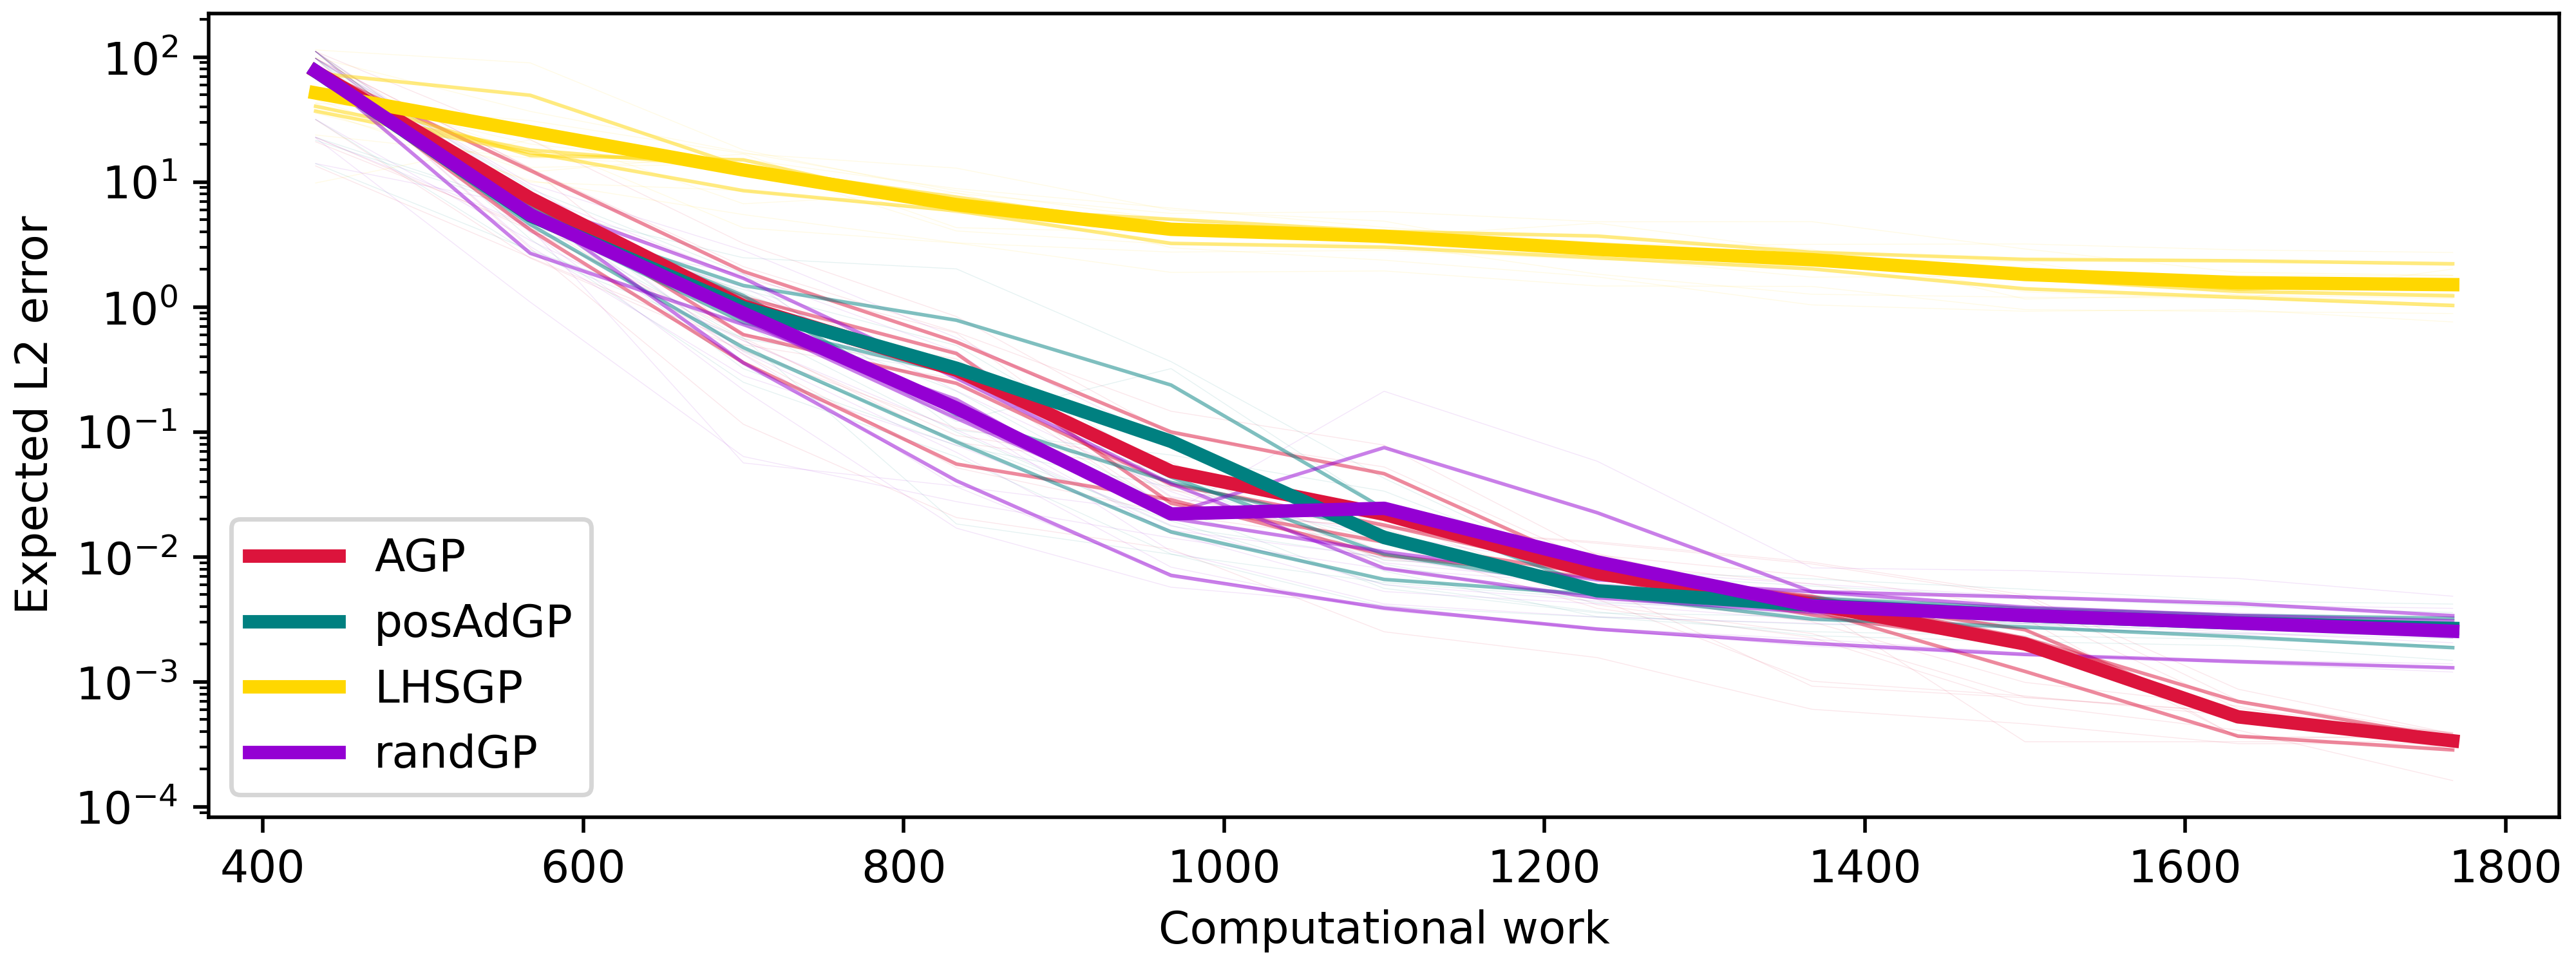
\includegraphics[width=0.8\textwidth]{results/pictures/d6/GP_res.png}
\end{center}
\caption{Convergence rates for the GP expected error over computational budget for the four considered strategies on the 6d example. The thinner lines represent a single run, the lines of median thickness represent the average over the 4 random seed for each measurement and the thickest lines represent the average over the whole 12 runs.}
    \label{fig:6dGPconv}
\end{figure}

The convergence curves resulting from the different training strategies with the above configuration are shown in Figure~\ref{fig:6dGPconv}.
In this example, we observe that, despite an overall higher error level, the relative performance of the different strategies is similar to the previous experiment; the position-adaptive strategies \texttt{posAdGP} and \texttt{randGP} stall at an error level of $10^{-3}$, while \texttt{AGP} is able to reach the target threshold $\texttt{tol}$ before the maximum number of iterations and \texttt{LHSGP} is unable to reduce the expected error significantly.
In contrast to the previous example, \texttt{AGP} is closer to the fixed-tolerance strategies \texttt{posAdGP} and \texttt{randGP} in terms of expected error per budget, but also spends considerably less budget than the previous experiment: both of these effects can be due to the higher likelihood standard deviation $\sigma$, here set to $2\cdot 10^{-2}$ in contrast to $10^{-2}$ in the previous example, which possibly makes the need for higher-accuracy evaluations less pressing.
This can also be seen in the lower number of iterations where no new candidate is selected, as shown in Table~\ref{tab:6dGP-recap}.
Another considerable difference is that \texttt{LHSGP} performs significantly worse than the other strategies, likely due to the higher dimensionality of the parameter space which makes evenly spaced sampling less effective.

\begin{table}[H]
    \begin{centering}
    \begin{tabular}{ccccc}
    \toprule
        & $E$   & $W$ & Training points    & Iterations \\ 
        \midrule
        \texttt{AGP}  
        & 0.0003 & 1734 & 31.9  &  23.1   \\
        \texttt{posAdGP}
        & 0.0021 & 1767 & 53    & 40   \\
        \texttt{randGP}
        & 0.0019 & 1767 & 53    & 40 \\
        \texttt{LHSGP}
        & 1.1770 & 1767 &  53   & 40   \\
    \bottomrule
    \end{tabular}
    \caption{Status of the training after the final iteration of different strategies for the GPR surrogate, 6d example. The average values over the 12 runs for the final error level $E$, total computational work $W$, the final number of points in the training set and the number of iterations necessary to terminate the training are provided.
    }
    \label{tab:6dGP-recap}
\end{centering}
\end{table}

For the LR we tried default configuration parameters similar to the previous one: after setting the halting threshold to $\texttt{tol} = \sigma \cdot \frac{\text{dim} \mc Y }{1.5} = 0.6$, we sampled every $N_{\text{sample}} = 5 $ iterations and set the number of walkers to $n_w = 64$.
The initial design consists of 13 points selected through LHS with default tolerance $\tau_d = 3 \cdot 10^{-2}$; we perform a maximum of $J_{\max} = 8 \cdot N_{\text{samples}} = 40$ iterations and at Step 3 of the algorithm we assign $\Delta W_j = \tau ^{-\frac{l}{r}}$ computational budget, using the default value $\tau= \tau_d$ for the first $2\cdot N_{\text{samples}}= 10$ iterations and then again halving it every $N_{\text{sample}}$ iterations if the expected error has not reduced by a factor 2 compared to the $N_{\text{sample}}$-th latest iteration, i.e. if $\frac{E(D(\mc D_j))}{E(D(\mc D_{j-N_{\text{sample}}}))} > \frac{1}{2}$.

This setup resulted in a poor performance for all strategies, as shown in Figure~\ref{fig:6dLRconv}, with \texttt{LHSLR} performing the worst but also the adaptive strategies \texttt{ALR}, \texttt{posAdLR} and \texttt{randLR} being unable to reduce the expected error significantly; moreover in the last iterations \texttt{ALR} spends considerably more budget than the fixed-tolerance strategies, resulting in a total computational work of 6766 for all of the runs as it tries to adaptively reduce the default tolerance $\tau_d$ but the expected error does not reduce correspondingly.
To try to improve the performance, we tried to lower the default tolerance $\tau_d$ to $10^{-3}$ and consider more iterations with $N_{\text{sample}} =  6$ and $J_{\max} = 9 \cdot N_{\text{sample}} $ in order to improve the results of all strategies, but this did not significantly improve the overall performance of any the considered strategies resulting in a lower error level but with convergence curves similar to the ones depicted in Figure~\ref{fig:6dLRconv}; despite the higher computational budget all strategies and runs were unable to reach the threshold \texttt{tol} and achieve convergence, with even the better runs not obtaining an error level below 1.

\begin{figure}[H]
\begin{center}
    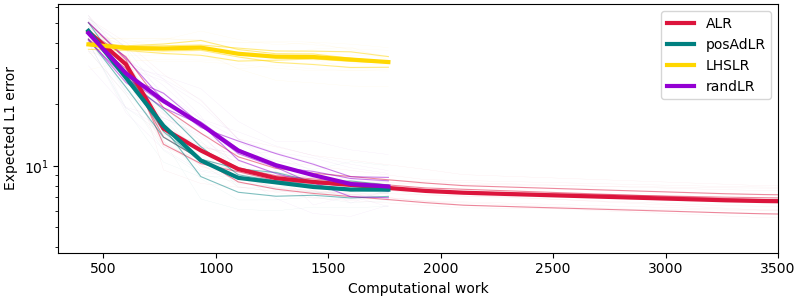
\includegraphics[width=0.8\textwidth]{results/pictures/d6/LR_res.png}
\end{center}
\caption{Convergence rates for the LR expected error over computational budget for the four considered strategies on the 6d example. The thinner lines represent a single run, the lines of median thickness represent the average over the 4 random seed for each measurement and the thickest lines represent the average over the whole 12 runs. The computational budget axis was truncated at 3300 as the budget spent by \texttt{ALR} far exceeds the ones from other strategies. }
    \label{fig:6dLRconv}
\end{figure}


The failure of LR on this problem can be attributed to the nature of the forward model; in fact, due to the rapid decay of the solution~\eqref{eq:diffusion-solution}, the steepness of every component varies greatly over the parameter space, and moreover the flatter and steeper regions are distinct for each component.
For a component $j$ of $y$, let $(t,x)$ being the corresponding time and sensor position.
Then, the Lipschitz constant for $y^{(j)}(x_p,x_n) = f(t,x;x_p,x_n)$ is given by 
\begin{align*}
    L^{(j)} = \max_{(x_p,x_n)\in\Theta}& \left\| \partial_{x_p,  x_n} y^{(j)}(x_p,x_n) \right\|_\infty  =
    \max_{x_p\in[-1,1]^3} \left\| \partial_{x_p} f(t,x;x_p,0) \right\|_\infty  =\\
    &\qquad \qquad= \max_{x_p\in [-1,1]^3} \left| \frac{50}{(4 \pi t)^{\frac{3}{2}}}\exp \left( - \frac{\norm{x-x_p}_2^2}{4t}\right) \frac{x^{(1)}-x_p^{(1)}}{4t} \right| 
    = \frac{100}{(8\pi)^{\frac{3}{2}}} e^{-\frac{1}{2}} t^{-2},
\end{align*}
where for symmetry reasons we can consider the derivative with respect to the first component of $x_p$ only, as the maximum is the same for all components of $\partial_{x_p, x_n} f(t,x;x_p,x_n)$, being obtained for component $h$ of $\partial_{x_p} f(t,x;x_p,x_n)$ in $x_p = x \pm \sqrt{2t} \cdot e_h$, with $e_h$ being the $h-$th vector of the canonical base of $\R^3$, and similarly for $x_n$.
Note that for any $(t,x) \in \mc S$ and $h \in \{1,2,3\}$, one between $(x + \sqrt{2t} e_h, \tilde x)$ and $(x - \sqrt{2t} e_h, \tilde x)$ is inside $\Theta$ for any $\tilde x \in [-1,1]^3$.

For $t=0.3$ and $t=0.5$ this results in a ground-truth global Lipschitz constant of approximately $ 5.3$ and $1.9$ for the respective components of the surrogate model.
However, in all components the minimum value of the local Lipschitz constant can go well below 0.1, and large portions of the parameter space can be covered with a significantly smaller Lipschitz constant.
This kind of behavior is extremely difficult to capture with a LR surrogate, which considers a global Lipschitz constant for every component of the forward model, as the surrogate requires a great number of points in order to be able to reduce the uncertainty of its prediction in the flatter region of each component.\medskip

The comparison of the performance of the GPR and LR surrogates is shown in Table~\ref{tab:6d-comparison}, where we can see that the performance of GPR is considerably better than that of LR; the best performance from an LR-based strategy is the one from \texttt{ALR}: but even for the fully-adaptive strategy strategy the corresponding estimates are unreliable and substantially 
wrong, and result being around as accurate as the ones provided by \texttt{LHSGP} for a smaller computational cost.
Regarding GPR-based strategies, two observations can be made.
First, the actual error values confirm the behavior suggested by the expected error curves, with the gap between \texttt{AGP} and the fixed-tolerance strategies being smaller, and the performance of \texttt{LHSGP} being far worse than in the 3d case.
Second, we can notice that while the median values achieved by \texttt{randGP} are on par with the other adaptive strategies, there is a considerably high maximum value for the error on the MAP and mean estimates.
As the standard deviation error does not display such phenomenon, this indicates that in some run \texttt{randGP} was misled and converged to the wrong posterior.

\begin{table}

    \begin{centering}
        
    
    \hspace*{-1.5cm}
    \begin{tabular}{ccccccccccccc}
    \toprule
        & \multicolumn{4}{c}{MAP error}  & \multicolumn{4}{c}{Posterior mean error} & \multicolumn{4}{c}{Posterior st. dev. error} \\ 
        & \multicolumn{4}{c}{$ \|p_\text{MAP} - \hat p _\text{MAP}\|_2 $}  & \multicolumn{4}{c}{$ \|p_\text{mean} - \hat p _\text{mean}\|_2 $} & \multicolumn{4}{c}{$\| \text{diag}(\Sigma_P) - \text{diag}( \hat \Sigma _P) \|_2$} \\ 
        & avg   & med   & min   & max   & avg   & med   & min   & max   & avg   & med   & min   & max \\
        \midrule
        \texttt{AGP}
        & 0.0086 & 0.0075 & 0.0029 & 0.0219
        & 0.0046 & 0.0036 & 0.0016 & 0.0105
        & 0.0935 & 0.0812 & 0.0657 & 0.1400 \\
        \texttt{posAdGP}
        & 0.0211 & 0.0164 & 0.0027 & 0.0637
        & 0.0270 & 0.0138 & 0.0013 & 0.1783
        & 0.0860 & 0.0845 & 0.0336 & 0.1383 \\
        \texttt{randGP}
        & 0.0511 & 0.0117 & 0.0051 & 0.3140
        & 0.0392 & 0.0062 & 0.0034 & 0.3378
        & 0.0998 & 0.0845 & 0.0336 & 0.1860 \\
        \texttt{LHSGP}
        & 0.2960 & 0.3019 & 0.1498 & 0.4543 
        & 0.2535 & 0.2439 & 0.0854 & 0.4684
        & 0.1229 & 0.1248 & 0.0226 & 0.2303 \\
        \texttt{ALR}
        & 0.3017 & 0.3139 & 0.1830 & 0.4252
        & 0.3021 & 0.3030 & 0.1383 & 0.4348
        & 0.0653 & 0.0657 & 0.0259 & 0.1099 \\
        \texttt{posAdLR}
        & 0.4045 & 0.3933 & 0.1955 & 0.6292
        & 0.3902 & 0.3541 & 0.1867 & 0.5732
        & 0.0655 & 0.0496 & 0.0191 & 0.1144 \\
        \texttt{randLR}
        & 0.5490 & 0.5420 & 0.3975 & 0.7604
        & 0.5563 & 0.5361 & 0.3867 & 0.7746
        & 0.0492 & 0.0423 & 0.0167 & 0.1089\\
        \texttt{LHSLR}
        & 0.6616 & 0.6180 & 0.3113 & 1.0597
        & 0.6257 & 0.6539 & 0.3246 & 0.9277
        & 0.2767 & 0.2836 & 0.0717 & 0.4703\\
        
    \bottomrule
    \end{tabular}
    \caption{Average, median, minimum and maximum of the absolute error on the MAP estimate, posterior mean and component-wise posterior standard deviation on each component over the 12 runs with default configuration.
    As for Table~\ref{tab:3d-comparison} the analytically available ground truth is used to compute the true quantities $p_\text{MAP}$, $p_\text{mean}$ and $\Sigma_P$, which are then compared with the surrogate-based estimates $\hat p_\text{MAP}$, $\hat p_\text{mean}$ and $\hat \Sigma_P$.
    }
    \label{tab:6d-comparison}
\end{centering}
\end{table}

\subsection{2d Finite Element example - Elastomechanics}\label{sec:FEexp}
For the third numerical experiment we consider a 2d elastomechanics problem, based on the equations of linear elasticity as introduced at the end of Section~\ref{sec:AdaFE}.
We consider a rectangular beam of length $L=4 m$ and quadratic cross-section of equal height and width $h=w=0.2 m$, constrained on the left and right sides, with a uniform downward load applied on the top side.
This conditions correspond to a Dirichlet boundary condition on the left and right sides, an inhomogeneous Neumann boundary condition on the top side and a homogeneous Neumann boundary condition on the rest of the beam.
Formally, our spatial domain is
\[
    \mc X = [0,L] \times [0,h] ^2 \in \R^3
\]
and we consider the homogeneous version of the Lamè-Navier equations~\eqref{eq:Navier-Lame} over $\mc X$
\[
    -2\mu \Delta u - \lambda \nabla (\nabla \cdot u) = 0,
\]
for Lamè parameters $\lambda, \mu$; the boundary conditions are given by
\[
    \begin{cases}
        u(x,y,z) = 0 & \text{ if } x = 0, L \\
        \partial_n u(x,y,z) = F & \text{ if } y = h \\
        \partial_n u(x,y,z) = 0 & \text{ otherwise}
    \end{cases}
\]
where $F = -5\cdot 10^6$ is a dimensionless quantity corresponding to a uniform load on the top.
We aim at identifying the Young's modulus $E$ and the Poisson's ratio $\nu$ of the material as given by Equation~\eqref{eq:material-parameters}.
We consider sensors placed in the center of the beam on the different sides, one at the top, one at the bottom, one on the left and one on the right
\[
    \mc S = \left\{ (2,0,0.1), (2,0.2,0.1), (2,0.1,0), (2,0.1,0.2) \right\} 
\]
and in each sensor we measure one component of the displacement field $u$ at the corresponding position: the vertical component for the top and bottom sensors and the horizontal component for the left and right sensors.
This results in a 4-dimensional measurement space $\mc Y = \R^4$ and a measurement operator \[
 \begin{gathered}
    H : H^1(\mc X;\R^3) \to \mc Y \\
    H(u) = S \begin{pmatrix}
     u^{(2)}(2,0,0.1)\\
     u^{(2)}(2,0.2,0.1)\\
     u^{(3)}(2,0.1,0)\\
     u^{(3)}(2,0.1,0.2) 
    \end{pmatrix} + a \in \R^4,
 \end{gathered}
\]
where the scaling diagonal matrix $S = \text{diag}(s_1, s_2, s_3, s_4)$ and the offset vector $a = (a_1,a_2,a_3,a_4)$ are added in order to center the model response into $[0,1]^4$.
We assume an original parameter space 
\[
    \hat \Omega = [90 \ GPa, 300 \ GPa] \times [0.1, 0.45] \subset \R^2 
\]
which for numerical stability we scale to $\Omega = [0,1]^2$ through an affine transformation.
As the forward model's image over the parameter space is in the order of $10^{-2}$ for the first two components and $10^{-6}$ for the last two, we set the scaling factors to $s_1 = s_2 = - \frac{100}{6}$ and $s_3 = - s_4 = 4 \cdot 10^5$ and the offset to $a_1 = a_2 = \frac{6}{100}$ and $a_3 = - a_4 = - 5 \cdot 10^{-7}$. \newline
We assume a Normal prior $\mc N(\frac{1}{2}, \frac{1}{6}I_2)$ over $\Omega$ and we consider a ground truth value for the parameters of $\hat p = (200 \ GPa, 0.25) \in \hat \Omega$, which are the material parameters of A36 steel.
The measurements are then generated by adding pseudorandom noise $N \sim \mc N (0, \sigma^2 I_4)$ with $\sigma = 10^{-2}$ to the forward model evaluation $y_\tau (p)$ for $p\in \Omega$ corresponding to the ground truth parameters $\hat p$ and with a tolerance of $\tau = 10^{-4}$.
Unlike the analytical examples, where we performed multiple runs in order to average over the randomly added noise, in this case we only perform one run for each strategy and surrogate, as the forward model is an actual FE model with non-negligible computational costs. \medskip

For the GPR surrogate we consider a default configuration similar to the one of the preceding examples, with the difference that we consider a default tolerance $\tau_{d,a}= 10^{-2}$ for the fully-adaptive \texttt{AGP} strategy and a default tolerance $\tau_{d,f} = 10^{-3}$ for the fixed-tolerance strategies.
We set the halting threshold to $\texttt{tol} = \sigma^2 \cdot \frac{\text{dim} \mc Y }{20} = 2\cdot 10^{-5}$, while sampling every $N_{\text{sample}} = 2$ iterations with an ensemble composed of $n_w = 16$ walkers.
For each strategy, the initial design comprises of $3$ points selected through LHS and evaluated with the default tolerance corresponding to the strategy; we perform a maximum of $J_{\max} = 10 \cdot N_{\text{samples}} = 20 $ iterations.
For the tolerance problem in \texttt{AGP}, we assign the budget $\Delta W_j = \tau ^{-\frac{l}{r}}$ using the default value $\tau= \tau_{d,a}$ for the first $2\cdot N_{\text{samples}} = 4$ iterations and then every $N_{\text{sample}}$ iterations we have $\tau$ if the expected error has not reduced by a factor 4 compared to the $N_{\text{sample}}$-th latest iteration, i.e. if $\frac{E(D(\mc D_j))}{E(D(\mc D_{j-N_{\text{sample}}}))} > \frac{1}{4}$.\medskip

\begin{figure}[H]
    \begin{center}
        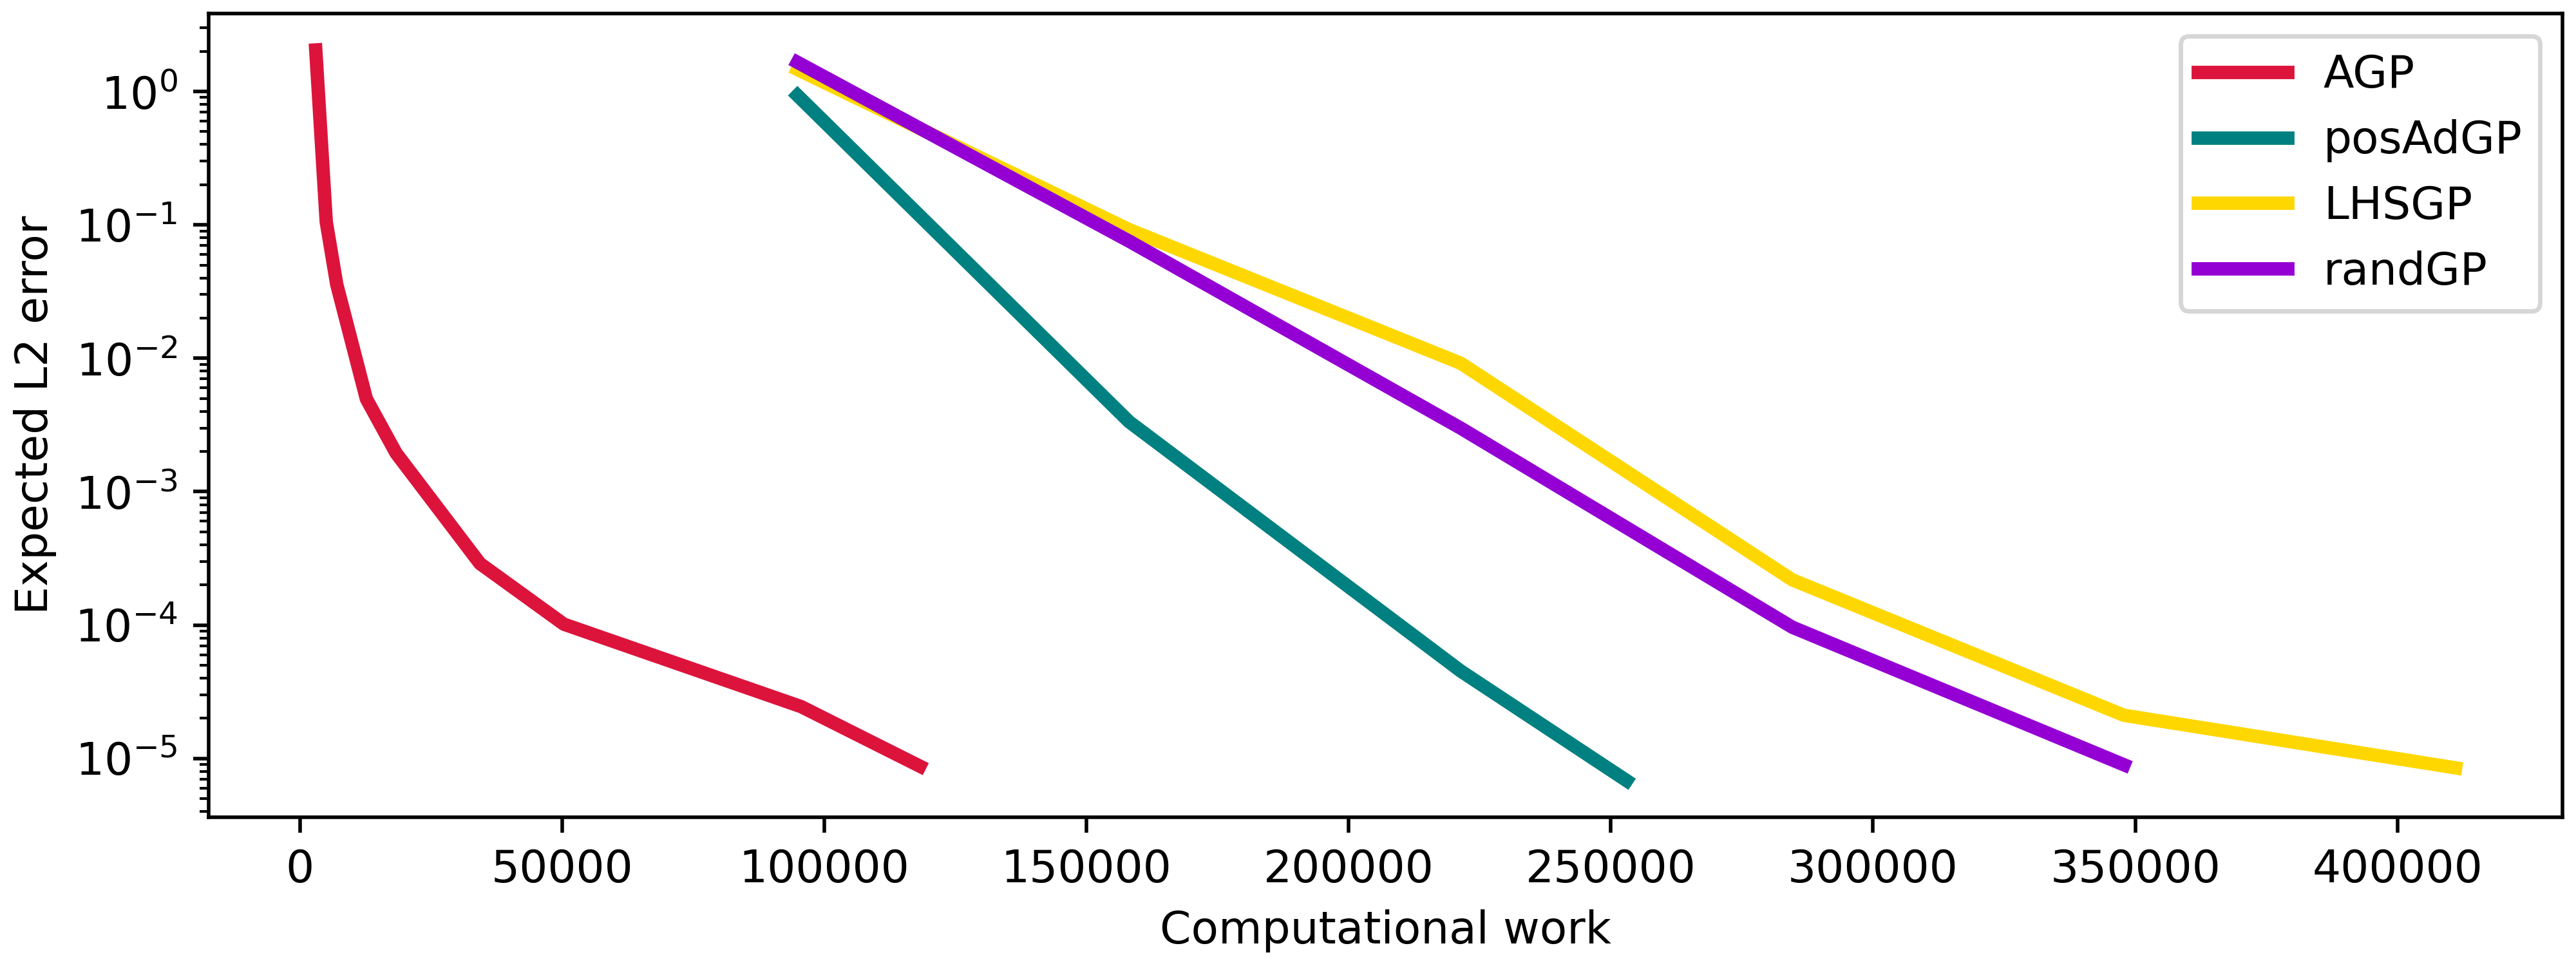
\includegraphics[width=0.8\textwidth]{results/pictures/d2/GP_res.png}
    \end{center}
    \caption{Convergence rates for the GP expected error over computational budget for the four considered strategies on the 2d FE example. A single line is plotted as a single measurement with a single random seed is used for each strategy.}
        \label{fig:FE-GP-convergence}
\end{figure}

Picture~\ref{fig:FE-GP-convergence} depicts the convergence curves for the GPR expected error over computational budget for the different strategies, while Table~\ref{tab:FE-GP-recap} summarizes the status of the training after the final iteration of the different strategies.
We observe that all strategies reach the halting threshold before the maximum number of iterations, included \texttt{LHSGP}, with the high accuracy strategies converging extremely rapidly; this success is likely due to the low dimensionality of the parameter space, which allows for a good coverage of the parameter space with relatively few high-accuracy points.
Moreover, we can see that \texttt{AGP} is able to reach the halting threshold with a significantly lower computational budget but higher number of points than the fixed-tolerance strategies.
Finally, we note that \texttt{randGP} performs worse than \texttt{posAdGP}, around at the level of \texttt{LHSGP}.
\begin{table}[H]
    \begin{centering}
    \begin{tabular}{ccccc}
    \toprule
        & converged   & $W$ & Training points    & Iterations \\ 
        \midrule
        \texttt{AGP}  
        & yes & 118196 &  15   &  16  \\
        \texttt{posAdGP}
        & yes & 252982 &  8   &  5  \\
        \texttt{randGP}
        & yes & 347851 &  11   &  8  \\
        \texttt{LHSGP}
        & yes & 411096 &  13   &  10  \\
    \bottomrule
    \end{tabular}
    \caption{Status of the training after the final iteration of different strategies for the GPR surrogate, FE example. For the single run performed the convergence status, total computational work $W$, the final number of points in the training set and the number of iterations necessary to terminate the training are provided.
    }
    \label{tab:FE-GP-recap}
\end{centering}
\end{table} 

For the LR surrogate we do similarly as done for the GPR surrogate, utilizing different tolerances for the fully-adaptive strategy \texttt{ALR} and the fixed-tolerance strategies \texttt{posAdLR}, \texttt{randLR} and \texttt{LHSLR}; we use a default tolerance $\tau_{d,a}= 10^{-2}$ for \texttt{ALR} and a default tolerance $\tau_{d,f} = 10^{-3}$ for the others.
The halting threshold is set to $\texttt{tol} = \sigma \cdot \frac{\text{dim} \mc Y }{1.5} = 2.\bar 6 \cdot 10^{-2}$, we sample every $N_{\text{sample}} = 3$ iterations and set the number of walkers to $n_w = 16$.
The initial design consists of $5$ points selected through LHS with the default tolerance corresponding to the strategy; we perform a maximum of $J_{\max} = 7 \cdot N_{\text{samples}} = 21 $ iterations and for the tolerance problem at Step 3 of the algorithm for \texttt{ALR} we assign $\Delta W_j = \tau ^{-\frac{l}{r}}$ using the default value $\tau= \tau_{d,a}$ for the first $2\cdot N_{\text{samples}} = 6$ iterations and then every $N_{\text{sample}}$ iterations we have $\tau$ if the expected error has not reduced by a factor 2 compared to the $N_{\text{sample}}$-th latest iteration, i.e. if $\frac{E(D(\mc D_j))}{E(D(\mc D_{j-N_{\text{sample}}}))} > \frac{1}{2}$.\medskip

\begin{figure}[H]
    \begin{center}
        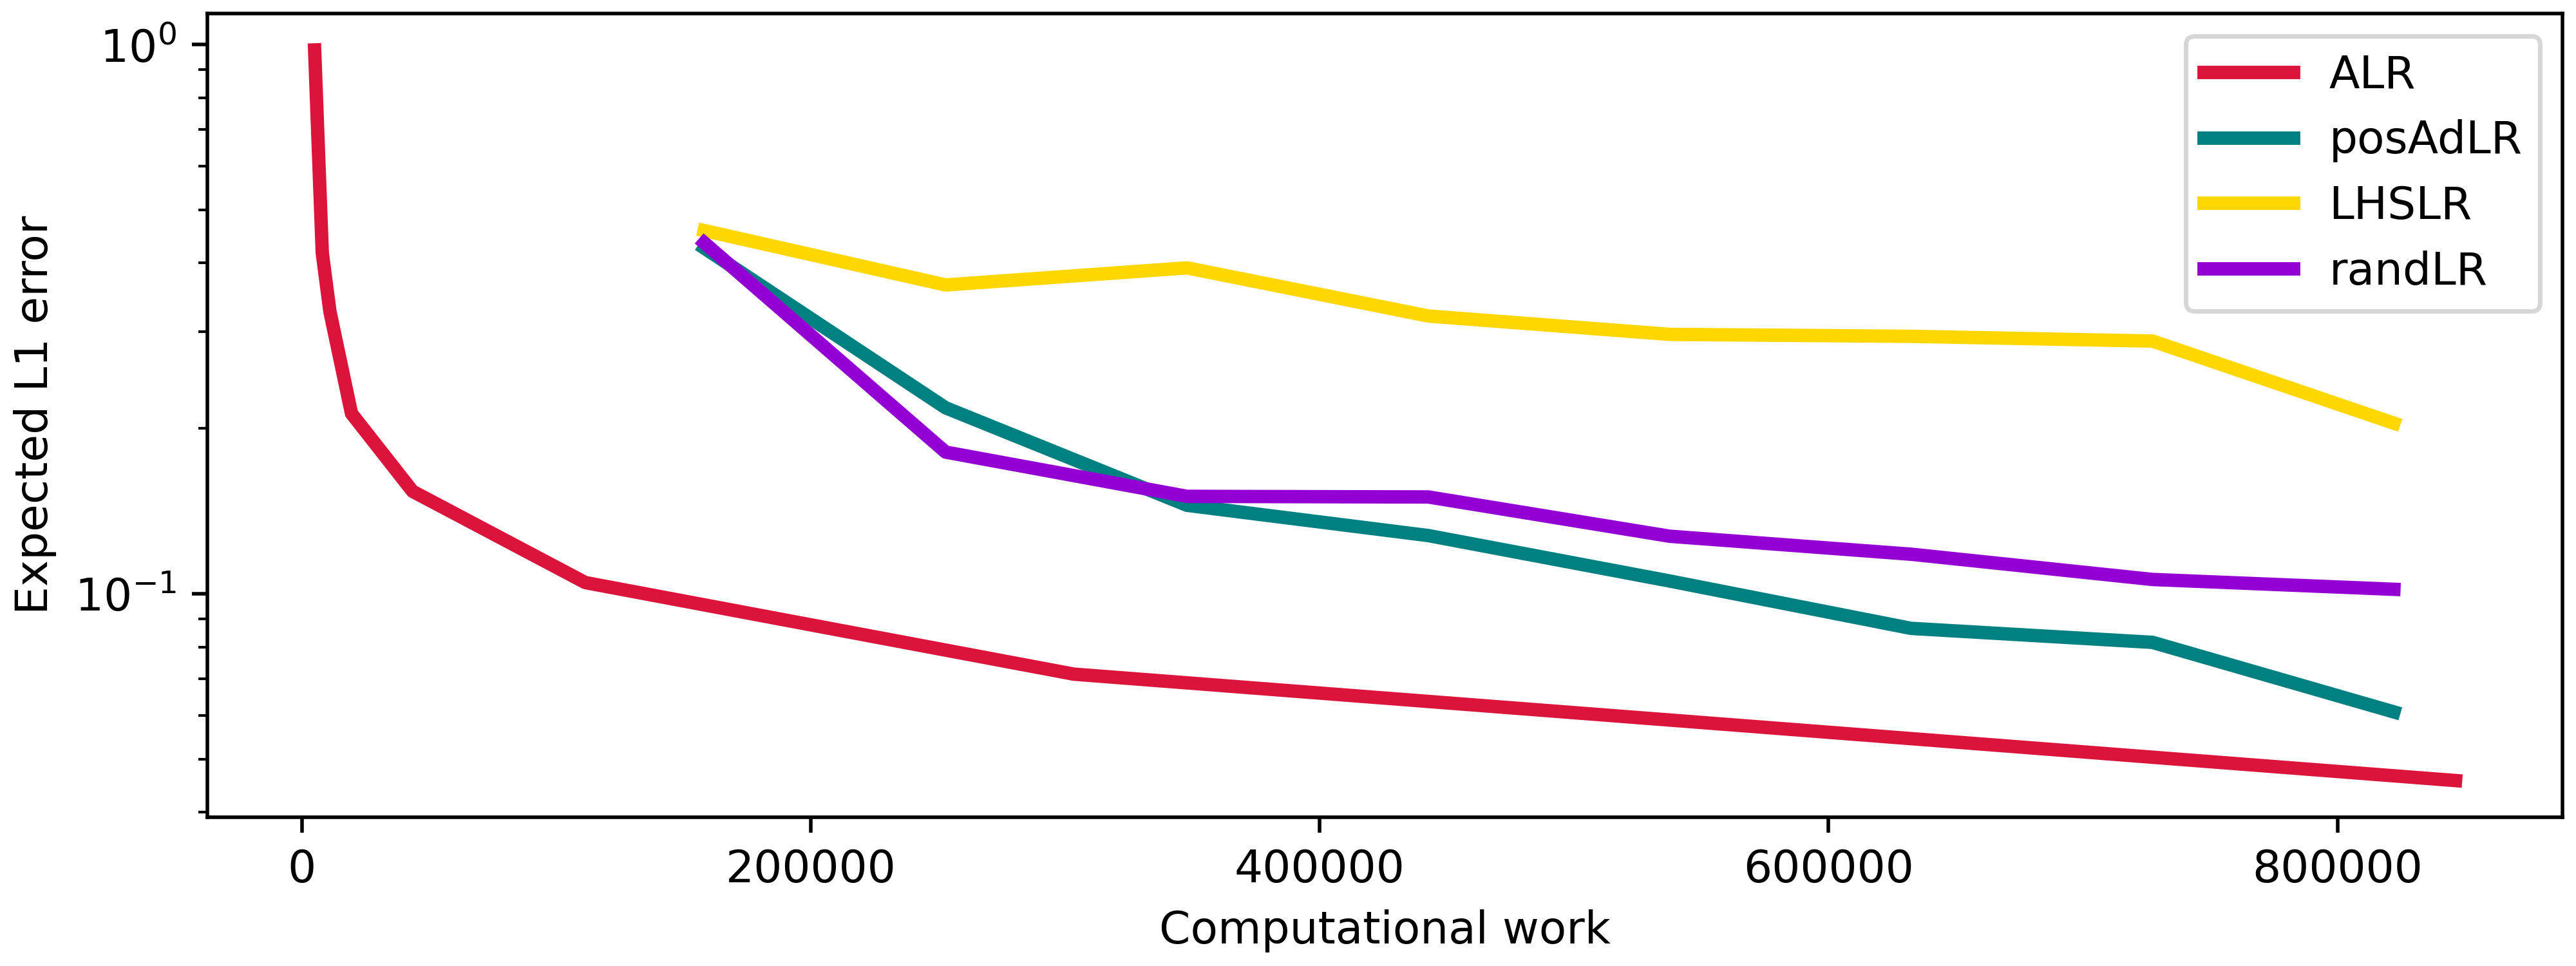
\includegraphics[width=0.8\textwidth]{results/pictures/d2/LR_res.png}
    \end{center}
    \caption{Convergence rates for the LR expected error over computational budget for the four considered strategies on the 2d FE example. A single line is plotted as a single measurement with a single random seed is used for each strategy.}
        \label{fig:FE-LR-convergence}
\end{figure}

The expected error over computational budget curves for the LR surrogate are shown in Picture~\ref{fig:FE-LR-convergence}, while Table~\ref{tab:FE-LR-recap} summarizes the status of the training after the final iteration of the different LR-based strategies. 
Unlike for the GPR-based strategies we observe that all strategies do not reach the halting threshold before the maximum number of iterations, included \texttt{ALR}; the error level remains high for all strategies, with \texttt{LHSLR} in particular struggling to reduce the expected error at all and \texttt{randLR} performing significantly worse than the other adaptive strategies.
In this example, the performance of \texttt{ALR} and \texttt{posAdLR} is not totally unsatisfying, as they are able to reduce the expected error to an order of $10^{-2}$, but the computational cost is considerably higher than the one of the GPR-based strategies without meeting the halting threshold.

\begin{table}[H]
    \begin{centering}
    \begin{tabular}{cccccc}
    \toprule
        & converged   & E & $W$ & Training points    & Iterations \\ 
        \midrule
        \texttt{AGP}  
        & no & 0.0457 & 846425 &  25   &  21  \\
        \texttt{posAdGP}
        & no & 0.0609 & 822192 &  26   &  21 \\
        \texttt{randGP}
        & no & 0.1019 & 822192 &  26   &  21 \\
        \texttt{LHSGP}
        & no & 0.2043 & 822192 &  26   &  21 \\
    \bottomrule
    \end{tabular}
    \caption{Status of the training after the final iteration of different strategies for the GPR surrogate, FE example. For the single run performed the convergence status, final error level $E$, total computational work $W$, the final number of points in the training set and the number of iterations necessary to terminate the training are provided.
    }
    \label{tab:FE-LR-recap}
\end{centering}
\end{table} 

Finally, Picture~\ref{fig:FE-samples} shows the samples gathered from the different strategies for both the GPR and the LR-based strategies.
We see that, while all strategies correctly identify the region of the parameter space where the ground truth is located, the GPR-based strategies provide a considerably more precise posterior distribution, with the samples being more concentrated around the ground truth and with a lower variance.
Among the LR-based strategies, \texttt{ALR} and \texttt{posAdLR} offer a better posterior representation than \texttt{randLR} and \texttt{LHSLR}, which provide an approximated posterior with high variance and multiple modes. 
\texttt{ALR} is rather close to the GPR-based strategies, but still displays an higher variance.

\begin{figure}[H]
    \begin{subfigure}[h]{0.45\linewidth}
    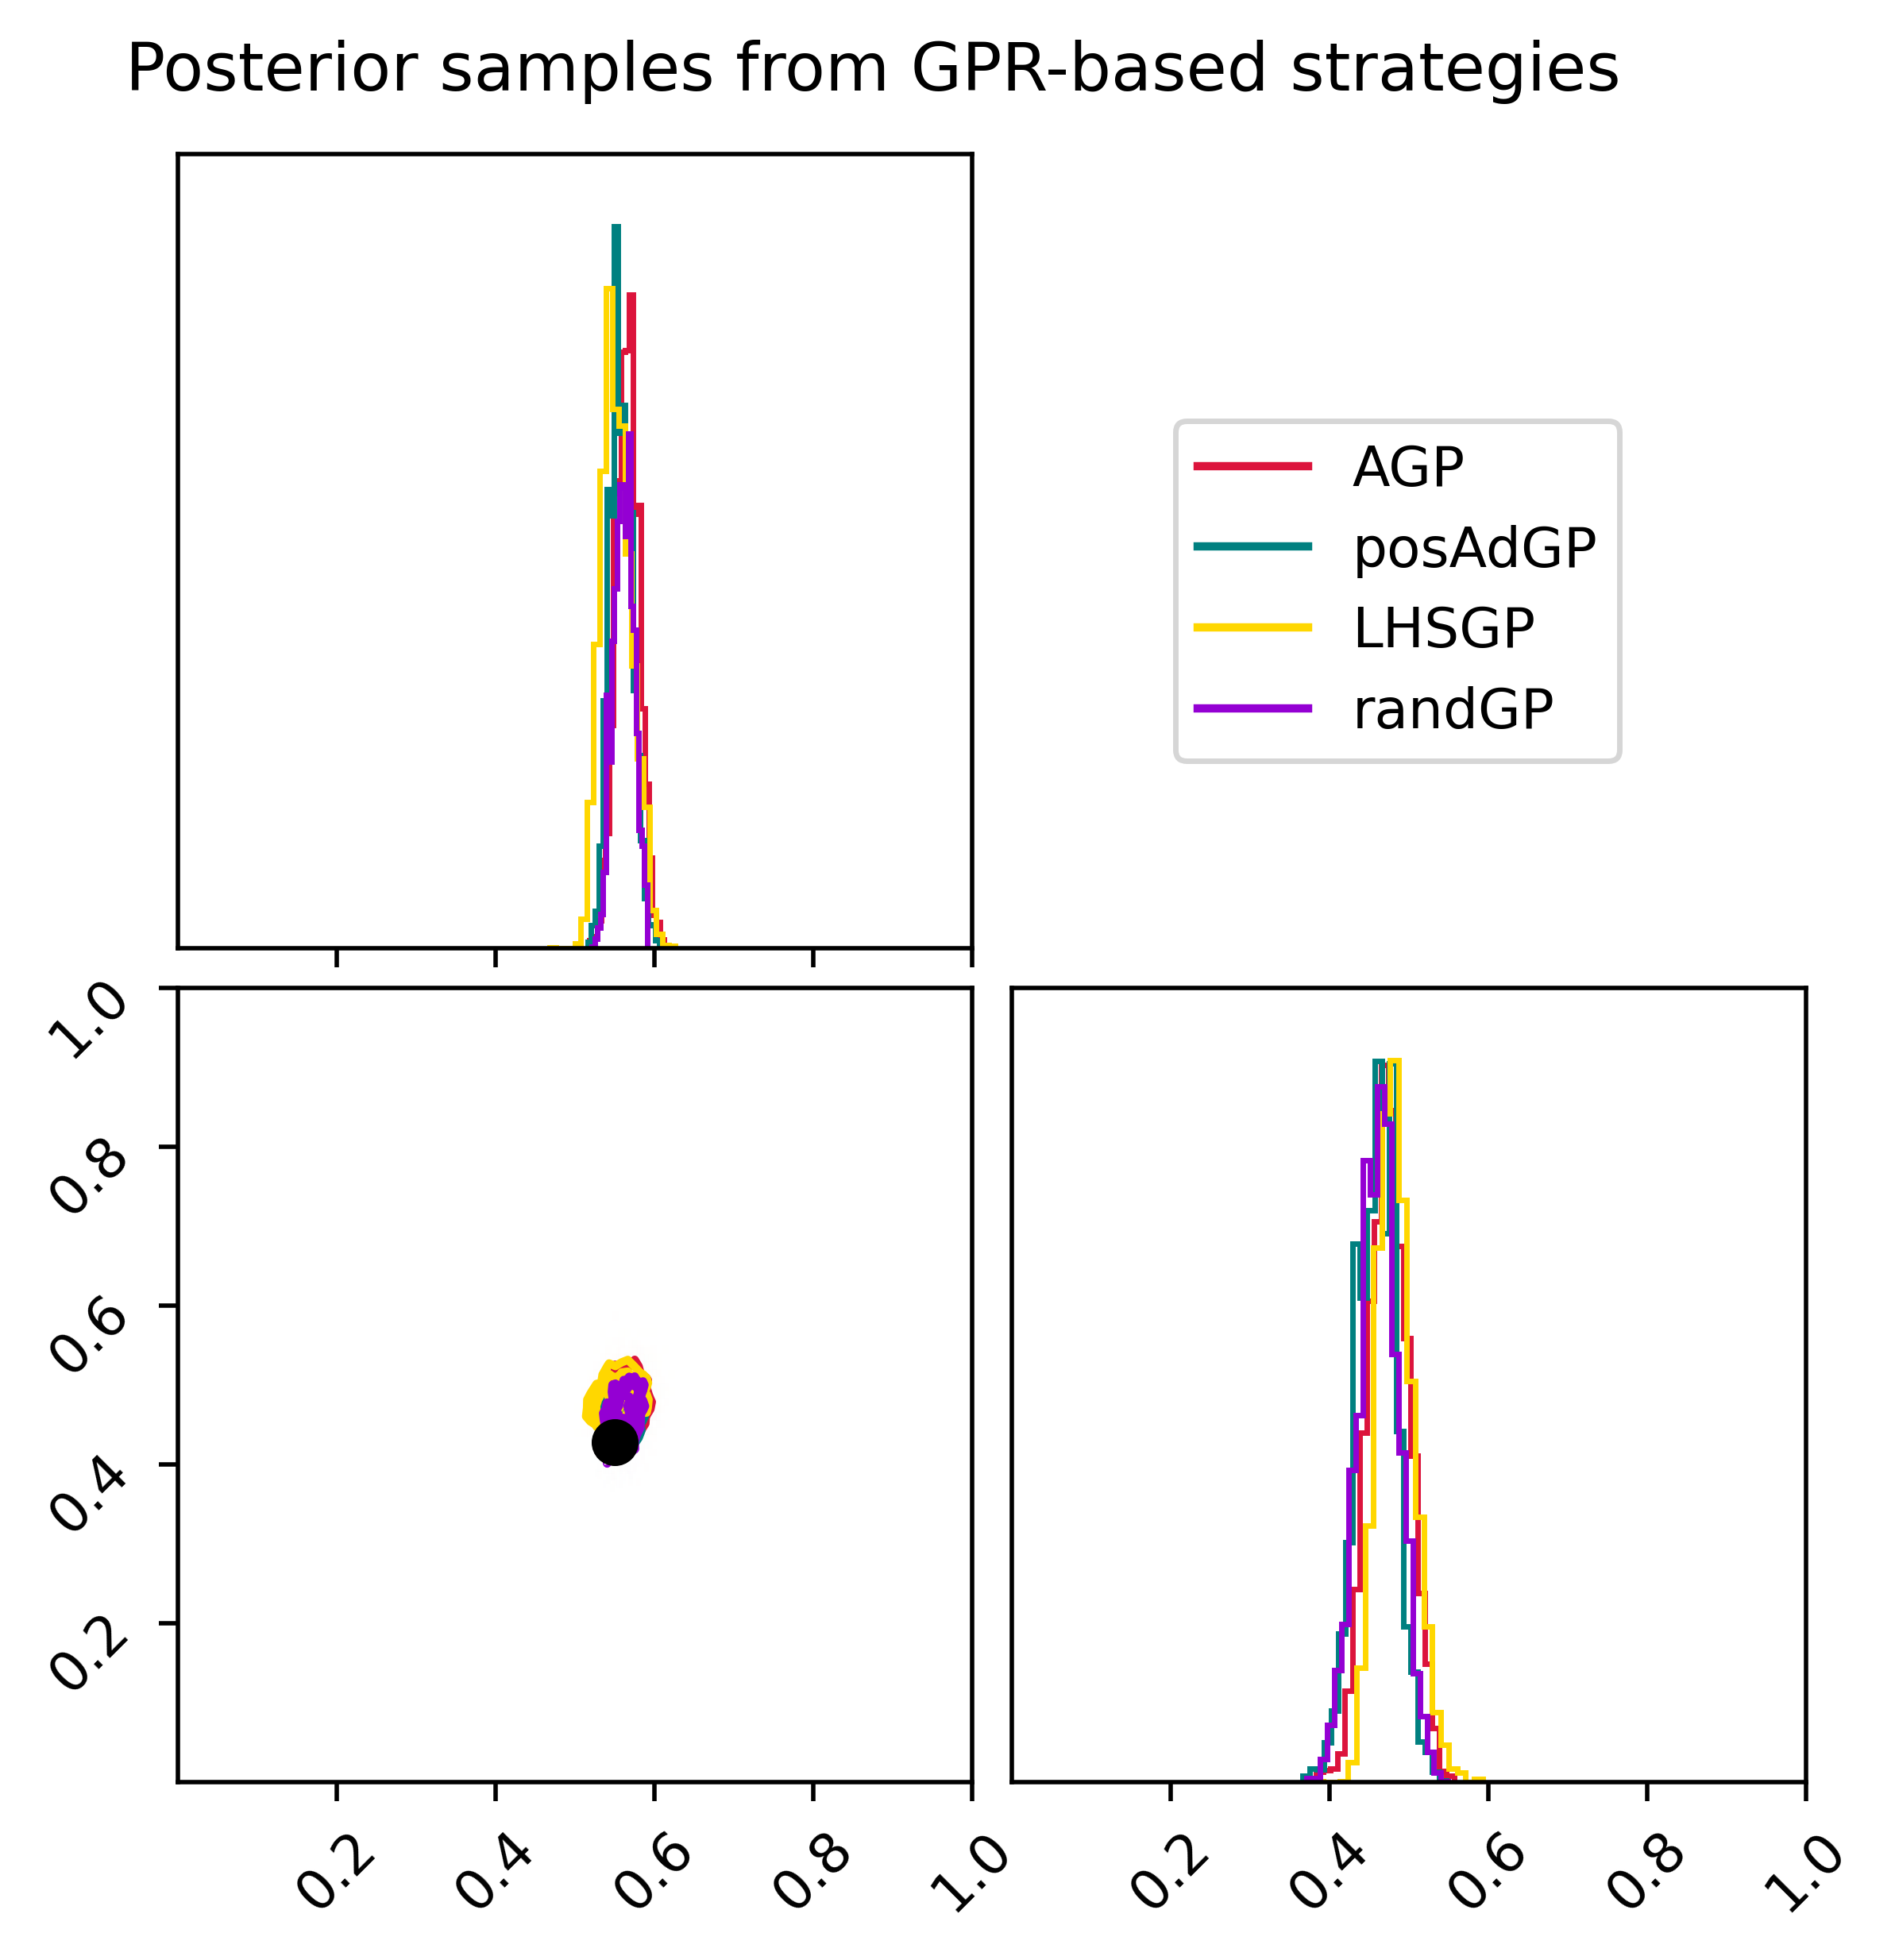
\includegraphics[width=\linewidth]{results/pictures/d2/GP_corner.png}
    \end{subfigure}
    \hfill
    \begin{subfigure}[h]{0.45\linewidth}
    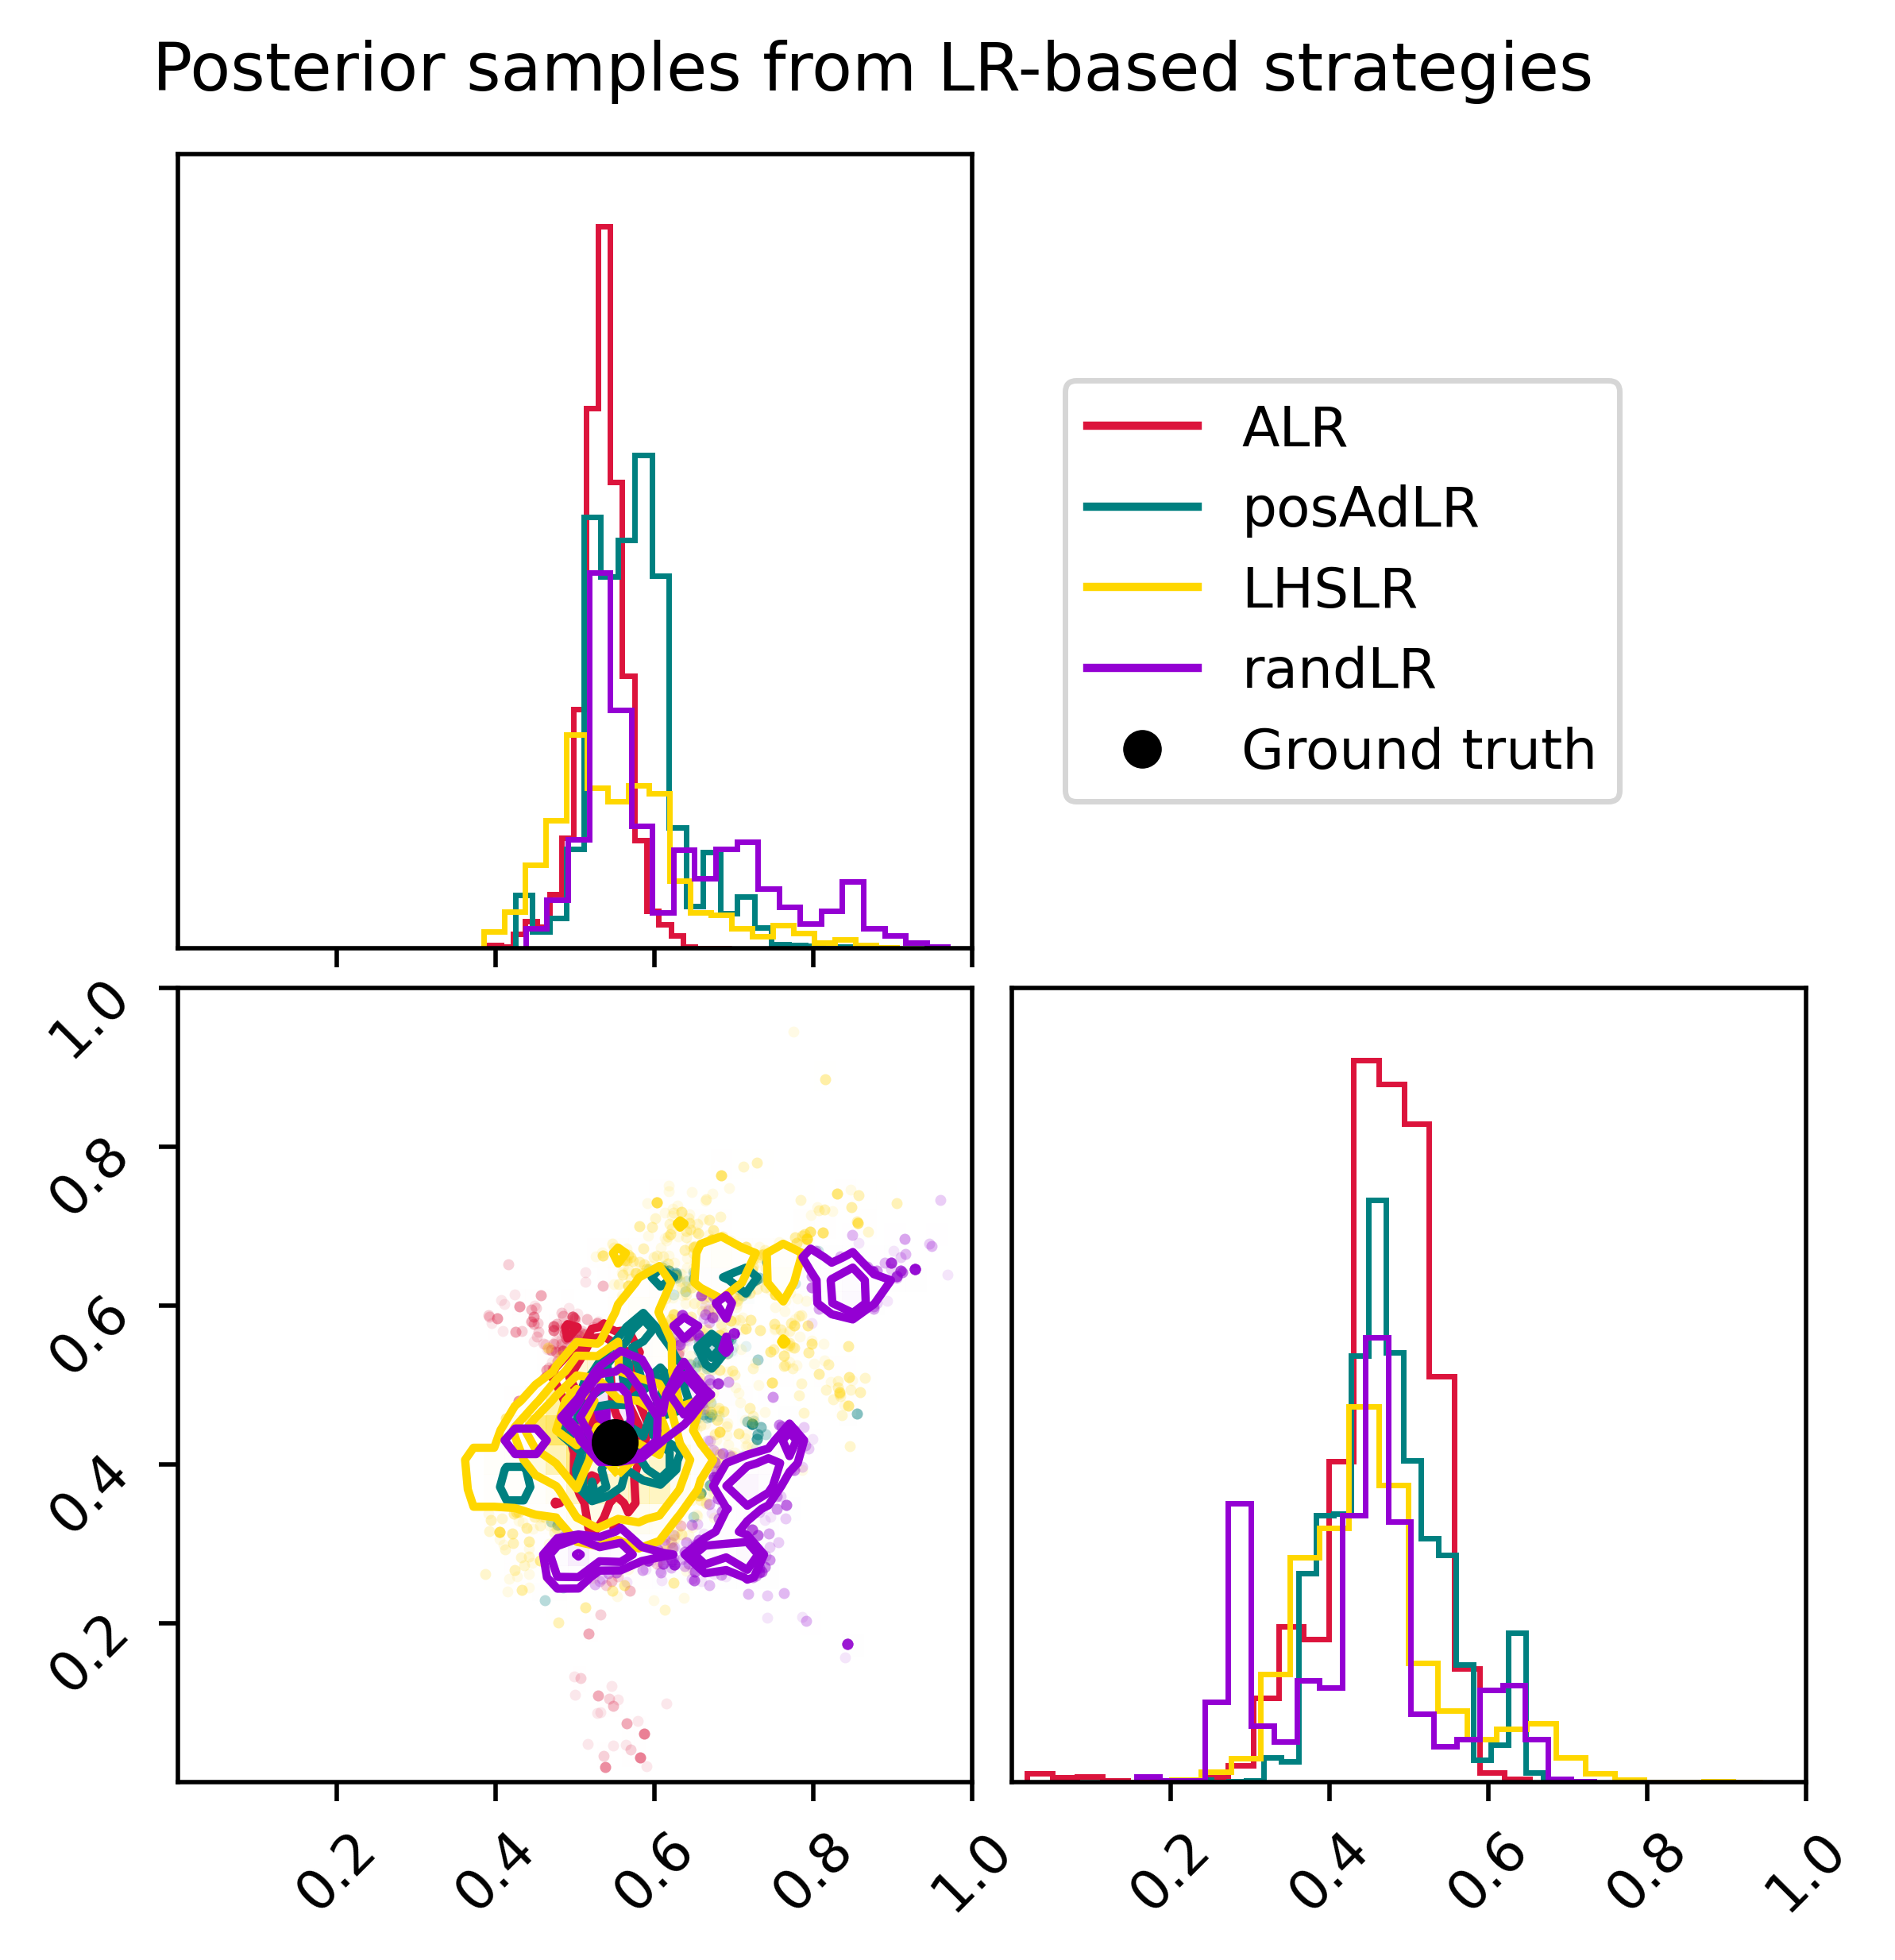
\includegraphics[width=\linewidth]{results/pictures/d2/LR_corner.png}
    \end{subfigure}%
    \caption{Gathered samples and ground truth $p$ on the scaled parameter space $\Theta$ for the GPR-based strategies (left) and the LR-based strategies (right), 2d FE example.}
    \label{fig:FE-samples}
\end{figure}


\subsection[Effects of covariance estimation]{Effects of the discretization noise's covariance estimation}\label{sec:cov-est}

To test the impact of the estimation of the discretization noise covariance $\Sigma_D^2$ on the performance of the surrogate, we utilize the data from the 3d and 6d analytical examples, where the discretization noise covariance is known.
First we test the error on the matrix 2-norm of the shrinkage covariance estimate $\hat \Sigma_d^2$ defined in Equation~\eqref{eq:shrinkage-estimator}; second, we test the effect of considering $\tau \hat \Sigma_d^2$ instead of diagonal noise $\tau I_{\text{dim}\mc Y}$ in GPR~\eqref{eq:GP-predictive} by training two GPR surrogates with $\hat \Sigma_d^2$ and $I_{\text{dim} \mc Y}$ as data noise covariances, and then comparing the resulting MAP estimates resulting from the surrogate-based posteriors.\medskip


To test the error on the covariance matrix $\Sigma_d^2$, we consider the covariance estimate $\hat \Sigma_d^2$ resulting from the final GPR surrogate trained with the \texttt{AGP} strategy for both the 3d and 6d examples, comparing the results with the true covariance $\Sigma_d^2$ over each run.
Table~\ref{tab:cov_est_err} summarizes the results of the covariance estimation for the two examples, showing the average, median, minimum and maximum of the error on the matrix 2-norm of the shrinkage covariance estimate $\hat \Sigma_d^2$ over the 25 runs for the 3d example and the 12 runs for the 6d example. \newline
The results show that, despite the high dimensionality of the covariance matrix $\Sigma_d^2$, being a $14\times 14$ matrix for the 3d example and a $30 \times 30$ matrix for the 6d example, the shrinkage covariance is able to estimate the covariance with a relative error of around 25\% for the 3d example and 45\% for the 6d example, in both cases providing a better estimate than the identity matrix $I_{\text{dim} \mc Y}$. \medskip

\begin{table}[H]

    \begin{centering}
        
    
    \hspace*{-1.5cm}
    \begin{tabular}{cccccc}
    \toprule
        & \multicolumn{4}{c}{Covariance estimate relative error}  & Identity relative error \\ 
        & \multicolumn{4}{c}{$ \|\hat \Sigma_d^2 - \Sigma_d^2\|_2 / \|\Sigma_d^2\|_2 $}  & $ \|I_{\text{dim} \mc Y} - \Sigma_d^2\|_2 / \|\Sigma_d^2\|_2 $ \\ 
        & avg   & med   & min   & max   &  \\
        \midrule
        3d example
        & 0.253 & 0.252 & 0.229 & 0.279
        & 0.344 \\
        6d example
        & 0.449 & 0.446 & 0.415 & 0.495 
        & 0.746 \\
        
    \bottomrule
    \end{tabular}
    \caption{Average, median, minimum and maximum of the relative error on the covariance estimate for the 3d and 6d examples, and relative distance of the identity matrix from the covariance estimate for comparison.
    }
    \label{tab:cov_est_err}
\end{centering}
\end{table}

We then test the effect of utilizing the covariance estimate $\hat \Sigma_d^2$ instead of the identity matrix $I_{\text{dim} \mc Y}$ for the GPR surrogate in an IP setting.
We train two GPR surrogates over the \texttt{AGP} training data gathered in Experiments~\ref{sec:3dexp} and~\ref{sec:6dexp}, one with the identity matrix and one with the covariance estimate $\hat \Sigma_d^2$, as discretization noise covariance, and then we compare the error on the MAP estimate given by the posteriors corresponding to the two surrogates.
The errors using $\hat \Sigma_d^2$ are the ones already reported in Table~\ref{tab:3d-comparison} and Table~\ref{tab:6d-comparison} for the 3d and 6d examples, respectively.
We compare them with the errors obtained using the identity matrix $I_{\text{dim} \mc Y } $ as noise covariance in Table~\ref{tab:cov_est_map}.

\begin{table}[H]
    \begin{centering}
        
    
    \begin{tabular}{ccccccccc}
    \toprule
        & \multicolumn{4}{c}{MAP error, $\hat \Sigma_d^2$} & \multicolumn{4}{c}{MAP error, $I_{\text{dim} \mc Y }$} \\ 
        & avg   & med   & min   & max   & avg   & med   & min   & max \\
        \midrule
        3d example   
        &0.0046 & 0.0039 & 0.0011 & 0.0086  &  0.0048 &  0.0042   &  0.0012  & 0.0091   \\
        6d example
        & 0.0086 & 0.0075 & 0.0029 & 0.0219  & 0.0091 &  0.0086   &  0.0028  & 0.0236   \\
    \bottomrule
    \end{tabular}
    \caption{Average, median, minimum and maximum of the absolute error on the MAP estimate using the covariance estimate $\hat \Sigma_d^2$ and the identity matrix $I_{\text{dim} \mc Y}$ as discretization noise covariance for the 3d and 6d examples, using the \texttt{AGP} training sets.
    }
    \label{tab:cov_est_map}
    \end{centering}
\end{table}

We can notice that the results using the covariance estimate $\hat \Sigma_d^2$ are slightly better than the ones using the identity matrix $I_{\text{dim} \mc Y}$ in both examples, but the difference does not significantly alter the performance of the surrogate.
This is likely due to the fact that the identity matrix $I_{\text{dim} \mc Y}$ is a good approximation of the discretization noise covariance $\Sigma_d^2$ as shown in Table~\ref{tab:cov_est_err}, in particular for the 3d example; moreover, the behavior of the GPR surrogate depends on a number of other factors, such as the kernel's structure and hyperparameters, which are likely to have a greater impact on the surrogate's performance than the choice of the discretization noise covariance.
However it is worth noticing that computing the covariance estimate $\hat \Sigma_d^2$ is computationally inexpensive whenever residuals estimates are available, rendering it potentially useful in contexts where the identity matrix is not a good approximation of the discretization noise covariance.